\documentclass[paper=a4,fontsize=12pt,oneside]{praca_mgr_pw_mod}

%dużo bibliotek ale niech zostają nie chce mi się poprawiać
\usepackage{graphicx}
\usepackage{caption}
\usepackage{subcaption}
\usepackage{amsfonts}
\usepackage{amsmath}
\usepackage{amsthm}
\usepackage{wrapfig}
%\usepackage{listings}
\usepackage{xcolor}
%\lstset{language=C}
\usepackage{fancyhdr}

\usepackage{moreverb}
\usepackage{booktabs}
\usepackage{eurosym}
\usepackage{indentfirst}
\usepackage{pdfpages}
\usepackage[utf8]{inputenc}
\usepackage{enumitem}
\usepackage{multirow}
\usepackage{rotating}
\usepackage{float}
\usepackage{tocloft}
\usepackage{color}
%\usepackage{xcolor,colortbl}
%\usepackage{mathtools}
%\usepackage{tablefootnote}
\usepackage{setspace}\setstretch{1.15} %było 1.2
\usepackage{tabularx}
%\usepackage{tgtermes}
\usepackage[titletoc]{appendix}
\usepackage{booktabs}
\usepackage{enumitem}
\setlist[1]{itemsep=-5pt}
\newcommand{\ra}[1]{\renewcommand{\arraystretch}{#1}}
\usepackage{color, colortbl}
\usepackage{array}
\usepackage{ragged2e}
\newcolumntype{P}[1]{>{\RaggedRight\hspace{0pt}}p{#1}}
%----------------------------------------------------------------------------------------
%	HYPERREFERENCES
%----------------------------------------------------------------------------------------
\usepackage{hyperref}  % backref linktocpage pagebackref

\usepackage{tabularx} % Better tables

\usepackage{enumitem} % Required for manipulating the whitespace between and within lists

\usepackage{polski}
\usepackage[utf8]{inputenc}

% LISTING
\usepackage{listings}
\usepackage{color}

\definecolor{mygreen}{rgb}{0,0.6,0}
\definecolor{mygray}{rgb}{0.5,0.5,0.5}
\definecolor{mymauve}{rgb}{0.58,0,0.82}

\lstset{ %
  backgroundcolor=\color{white},   % choose the background color; you must add \usepackage{color} or \usepackage{xcolor}
  basicstyle=\footnotesize,        % the size of the fonts that are used for the code
  breakatwhitespace=false,         % sets if automatic breaks should only happen at whitespace
  breaklines=true,                 % sets automatic line breaking
  captionpos=b,                    % sets the caption-position to bottom
  commentstyle=\color{mygreen},    % comment style
  deletekeywords={...},            % if you want to delete keywords from the given language
  escapeinside={\%*}{*)},          % if you want to add LaTeX within your code
  extendedchars=true,              % lets you use non-ASCII characters; for 8-bits encodings only, does not work with UTF-8
  frame=single,                    % adds a frame around the code
  keepspaces=true,                 % keeps spaces in text, useful for keeping indentation of code (possibly needs columns=flexible)
  keywordstyle=\color{blue},       % keyword style
  language=VHDL,                 % the language of the code
  morekeywords={*,...},            % if you want to add more keywords to the set
  numbers=left,                    % where to put the line-numbers; possible values are (none, left, right)
  numbersep=5pt,                   % how far the line-numbers are from the code
  numberstyle=\tiny\color{mygray}, % the style that is used for the line-numbers
  rulecolor=\color{black},         % if not set, the frame-color may be changed on line-breaks within not-black text (e.g. comments (green here))
  showspaces=false,                % show spaces everywhere adding particular underscores; it overrides 'showstringspaces'
  showstringspaces=false,          % underline spaces within strings only
  showtabs=false,                  % show tabs within strings adding particular underscores
  stepnumber=2,                    % the step between two line-numbers. If it's 1, each line will be numbered
  stringstyle=\color{mymauve},     % string literal style
  tabsize=2,                       % sets default tabsize to 2 spaces
  title=\lstname                   % show the filename of files included with \lstinputlisting; also try caption instead of title
}


\renewcommand\lstlistingname{Wydruk}
\renewcommand\lstlistlistingname{Wydruki}
\renewcommand\listfigurename{{\LARGE Rysunki}}
\renewcommand{\figurename}{Rys.}
\renewcommand\tablename{Tab.}

\renewcommand{\listtablename}{{\LARGE Tablice}}
\renewcommand{\bibname}{Literatura}


%    Abstract: \abstractname
%    Appendix: \appendixname
%    Bibliography: \bibname
%    Chapter: \chaptername
%    Contents: \contentsname
%    Index: \indexname
%    List of Figures: \listfigurename
%    List of Tables: \listtablename
%    Part: \partname
%    References: \refname

% Nie pozostawia na końcu wdów i sierot
\usepackage{lettrine}\sloppy %zakaz wydłużania lini (gdzy nie może złożyć) 
\clubpenalty=10000 %nie dieli wyrazów pomiędzy stronami 
\widowpenalty=10000 %nie pozostawia wdów i sierot pojedynczych 
\usepackage{fancyhdr}

\usepackage{pdfpages}

\usepackage{graphicx}
\usepackage{caption}
\usepackage{subcaption}

%---------------------------------------------------------------                
%TikZ config file - contains confuguration for use charts, plots, diagramflow...
% put file before document begining

\usepackage{tikz}			%inlcude always
\usepackage{verbatim}		%include always

%-------------------------------------------------------------------------------
% Circular arrows with text
%-------------------------------------------------------------------------------
\usetikzlibrary{decorations.text}
\newcommand*{\mytextstyle}{\sffamily\bfseries\color{black!85}}
\newcommand{\arcarrow}[8]{%
% inner radius, middle radius, outer radius, start angle,
% end angle, tip protusion angle, options, text
  \pgfmathsetmacro{\rin}{#1}
  \pgfmathsetmacro{\rmid}{#2}
  \pgfmathsetmacro{\rout}{#3}
  \pgfmathsetmacro{\astart}{#4}
  \pgfmathsetmacro{\aend}{#5}
  \pgfmathsetmacro{\atip}{#6}
  \fill[#7] (\astart:\rin) arc (\astart:\aend:\rin)
       -- (\aend+\atip:\rmid) -- (\aend:\rout) arc (\aend:\astart:\rout)
       -- (\astart+\atip:\rmid) -- cycle;
  \path[font = \sffamily, decoration = {text along path, text = {|\mytextstyle|#8},
    text align = {align = center}, raise = -0.5ex}, decorate]
    (\astart+\atip:\rmid) arc (\astart+\atip:\aend+\atip:\rmid);
}
%-------------------------------------------------------------------------------

%-------------------------------------------------------------------------------
% Inertial navigation system
%-------------------------------------------------------------------------------
\usetikzlibrary{shapes,arrows}
\usepackage{amsmath,bm}
\newcommand{\mx}[1]{\mathbf{\bm{#1}}} % Matrix command
\newcommand{\vc}[1]{\mathbf{\bm{#1}}} % Vector command
%-------------------------------------------------------------------------------

%-------------------------------------------------------------------------------
% State machine
%-------------------------------------------------------------------------------
\usetikzlibrary{arrows,automata}
%-------------------------------------------------------------------------------

%-------------------------------------------------------------------------------
% Computer science mindmap
%-------------------------------------------------------------------------------
\usetikzlibrary{mindmap,trees}
%-------------------------------------------------------------------------------

%-------------------------------------------------------------------------------
% Borrowers and lenders
%-------------------------------------------------------------------------------
\usetikzlibrary{arrows,positioning} 
\tikzset{
    %Define standard arrow tip
    >=stealth',
    %Define style for boxes
    punkt/.style={
           rectangle,
           rounded corners,
           draw=black, very thick,
           text width=6.5em,
           minimum height=2em,
           text centered},
    % Define arrow style
    pil/.style={
           ->,
           thick,
           shorten <=2pt,
           shorten >=2pt,}
}
%-------------------------------------------------------------------------------
\usetikzlibrary{arrows,decorations.pathmorphing,backgrounds,fit,positioning,shapes.symbols,chains}
%-------------------------------------------------------------------------------
   % odkomentuj jak chcesz pisać schematy w Latex i zainstaluj pakiet TikZ

\usepackage{polski}
\usepackage[utf8]{inputenc}

\begin{document}
\pagenumbering{gobble}
%----------------------------------------------------------------------------------------
%	PRE-CONTENT THESIS PAGES 	(na koniec odkomentować)
%----------------------------------------------------------------------------------------
	% Title Page

\begin{titlepage}


\begin{center}
\hfill \\
\vspace{0.1cm} 
\hfill \\
 

\includegraphics[height=4cm]{gfx/logo_pw.jpg}\hfill

\includegraphics[height=4cm]{gfx/logo_weiti.jpg}\\ \medskip % Picture
\large
\hfill
\vfill

\begingroup
{\Large Politechnika Warszawska} \\ 
{\Large Wydział Elektroniki i Technik Informacyjnych} \\ 
{\Large Instytut Systemów Elektronicznych} \\ \bigskip
\vfill
{\Huge \textbf{Tomasz Ferens}} \\ % Your name
{numer indeksu: 246156} \\ \bigskip
\vfill
{\large Praca Inżynierska} \\ \medskip % Picture
{\LARGE {\textbf{Szybka, Inteligentna kamera z interfejsem Ethernet.}}} \\ \bigskip % Thesis title
\endgroup
\vfill
%\hfill {nr albumu: 246289} \\ \bigskip % Thesis title
\hfill {Praca wykonana pod kierunkiem:} \\ % Your name 
\hfill {dr. inż. Grzegorza Kasprowicza} % Your name
\vfill
\vspace{3cm}

Warszawa, 2015



\end{center}


\end{titlepage} 	% Main title
	\cleardoublepage	
	% Abstract
\newpage
\pdfbookmark[1]{Abstract}{Abstract} % Bookmark name visible in a PDF viewer

\begingroup
\let\clearpage\relax
\let\cleardoublepage\relax
\let\cleardoublepage\relax

\hfill \\
\vspace{0.1cm} 
\hfill \\
%\chapter*{Streszczenie} % Abstract name
{\LARGE \textbf{Streszczenie \\ \vspace{0.5cm} \\ }}

Tytuł: \textbf{\textit{Szybka, Inteligentna kamera z interfejsem Ethernet.}} \\

\textit{W poniższej pracy zaprezentowany jest projekt szybkiej, inteligentnej kamery opartej na systemie wbudowanym Raspberry Pi 2 z układem SoC BCM2836 firmy Broadcom oraz modułem kamery RaspiCam -  sensor ov5647. 
Dzięki wydajnym podzespołom płyty Raspberry Pi 2 możliwe jest szybkie przetworzenie obrazu w celu detekcji wymaganego wzorca i wykonanie określonej akcji.
Moduł Ethernet umożliwia komunikację między użytkownikiem, a płytą za pomocą sieci internetowej.
Płyta pracuje pod kontrolą systemu Linux, dystrybucji Raspbian , na którym uruchamiana jest aplikacja napisana w języku C++.
W pracy przedstawiona jest jedna z wielu koncepcji wykorzystania inteligentnej kamery oraz jej praktyczna realizacja.} \\

Słowa kluczowe: \textbf{\textit{systemy wbudowane, wizja komputerowa, Ethernet, Internet of Things, Raspberry Pi 2, OV5647, OpenCV, Linux, przetwarzanie sygnałów. }} 
\\
\vspace{1cm} \\

{\LARGE \textbf{Abstract \\ \vspace{0.5cm} \\ }}

Title: \textbf{\textit{Fast, smart camera with Ethernet interface.}} \\

\textit{In this paper is presented project fast, smart camera based on embedded system Raspberry Pi 2 with SoC Broadcom BCM2836 and camera module RaspiCam - ov5647 sensor.
Thanks to the efficient hardware components of Raspberry Pi 2, it is possible to quickly process the image in order to detect the desired pattern and perform specific action.
Ethernet module enables communication between the user and the device via the Web.
The device is running under control of Linux system, distribution Raspbian used to run an application written in C ++.
The idea presented in this work is one of the many concepts of using smart camera and its practical implementation.} \\

Key words: \textbf{\textit{Embedded Systems, Digital Image Processing, Ethernet, Internet of Things, Raspberry Pi 2, OV5647, OpenCV, Linux, Signal Processing.}}

\endgroup			

\newpage		% Abstract
	\cleardoublepage
	% Title Page
\newpage
{
\vfill

%\begin{wrapfigure}[4]{Lh}{6cm}

\includegraphics[width=5cm]{gfx/Ferens.jpg} \\ \medskip 
%\end{wrapfigure}
\vspace{3mm} 
\hfill Imię i nazwisko: \textbf{Tomasz Ferens}  \\
\vspace{3mm} 
\hfill Specjalność: \textbf{Elektronika i Inżynieria Komputerowa}  \\ 
\vspace{3mm}   
\hfill Data urodzenia: \textbf{XX miesiąc 19XX r. }  \\ 
\vspace{3mm} 
\hfill Data rozpoczęcia studiów: \textbf{1 października 2011 r. }  \\ 
\vfill
\begin{center}
{ {\LARGE Życiorys} } \\ \bigskip
\end{center}

\vspace{2cm}
\hspace{1cm} Urodziłem się 5 grudnia 1992 roku w Białej Podlaskiej. W latach 2008--2011
uczęszczałem do~II Liceum Ogólnokształcącego im. Emilii Plater do klasy o~profilu matematyczno-informatycznym. W~2011 roku uzyskałem świadectwo dojrzałości i~rozpocząłem studia na~Wydziale Elektroniki i~Technik Informacyjnych Politechniki Warszawskiej na~makrokierunku Elektronika, Informatyka i Telekomunikacja. Po~czwartym semestrze studiów wybrałem
specjalizację Elektronika i Inżynieria Komputerowa. \\ 
\vfill
\vspace{4cm}
%\begin{center}
%{ {\LARGE Egzamin dyplomowy} }  \\ 
%\end{center}
%\vfill
%Złożył egazmin dyplomowy dn. \dotfill  \\ 
%Z wynikiem. \dotfill \\ 
%Ogólny wynik studiów \dotfill \\ 
%Dodatkowe wnioski i uwagi Komisji \dotfill \\ 
%.\dotfill \\
%.\dotfill \\ 
%.\dotfill \\ 
%\vfill
%\newpage
}			% Życiorys
	\cleardoublepage
	% Dedication

\thispagestyle{empty}

\pdfbookmark[1]{Dedication}{Dedication} % Bookmark name visible in a PDF viewer

\vspace*{18cm}

\begin{flushright}
\emph{Pragnę złożyć serdeczne podziękowania za okazaną pomoc \\ dr. inż. Grzegorzowi Kasprowiczowi} \\ \medskip
\end{flushright}


\medskip

\begin{flushright}
\emph{Pracę dedykuję Rodzicom jako wyraz wdzięczności za trud wychowania. \\ }\smallskip

\end{flushright} 	% Dedykacja podziękowanie
	\cleardoublepage						

	\pagenumbering{arabic}	
	\tableofcontents % Bookmark name visible in a PDF viewer
	\newpage
	\lstlistoflistings
	\listoftables
	\listoffigures

%----------------------------------------------------------------------------------------
%	CHAPTERS
%-----------------------------------------------------------------------------------	
	% Chapter 1

\chapter{Wprowadzenie} % Chapter title
%propedeutyka = «wiadomości wprowadzające do jakiejś dziedziny wiedzy» 
\label{ch:name} % For referencing the chapter elsewhere, use \autoref{ch:name}
 
\begin{flushright}
\emph{''Powszechnie wiadomo, że kamień potrafi myśleć. Na tym fakcie opiera się cała elektronika.''}

\textit{{\footnotesize (Równoumagicznienie, Terry Pratchett)}  }
\end{flushright}


Rozwój elektroniki, a szczególnie systemów mikroprocesorowych w ostatnich latach ma niebagatelny wpływ na niemal każdy aspekt naszego życia. Systemy te wraz z ewolucją są wykorzystywane już nie tylko do specjalnych zastosowań w wąskich dziedzinach, ale także jako elementy ułatwiające nam codzienne życie. Do jednych z wielu dziedzin, w których są kluczowe można zaliczyć min. : robotykę, motoryzację, medycynę, sport, tzw. inteligentne systemy. Obserwując zastosowania dzisiejszej elektroniki w obliczu społeczeństwa informacyjnego można stwierdzić trafność słów T. Pratchett'a. Powszechność elektroniki umożliwia jej obecność nawet w "kamieniach".

Pojęcie inteligentnych systemów w ostatnim czasie jest bardzo powszechne. Systemy te wyróżniają się tym, że zamiast wykonywania z góry założonego schematu działania są wyposażone w dodatkową inteligencję. Inteligencja ta daje dużo większe możliwości wykorzystania urządzenia, gdyż odpowiednio zastosowana daje możliwość odciążenia użytkownika z części zadań, lub nawet wykonania ich dużo sprawniej i dokładniej.
Jako, że wraz z rozwojem technologii możliwości układów SoC  wzrastają, przy niewielkich wciąż wymiarach, pozwala to zawrzeć w chipie module wiele podzespołów, takich jak  dedykowane układy graficzne, moduły komunikacji sieciowej, oraz inne podsystemy rozszerzające funkcjonalność układu.

Ponadto systemy wbudowane odgrywają znaczącą rolę szczególnie tam, gdzie niewielkie gabaryty urządzenia i niski pobór mocy są kluczowe.

Przykładem takiego systemu może być inteligenta kamera, której zadaniem jest detekcja  danego obiektu i podjęcie określonej przez projektanta akcji np. sterowania innym urządzeniem lub podzespołem, czy też tworzeniem statystyk.

\subsection*{Internet of Things}
Temat niniejszej pracy świetnie wpasowuje się w koncepcję tzw. Internetu Rzeczy (ang. Internet of Things- skr. IoT). Według której wszelkiego rodzaju urządzenia mogą stanowić jedną wielką sieć, pozwalającą sprawniej ze sobą wydajnie współpracować komunikując się ze sobą, wspólnie przetwarzając i wymieniając dane za pomocą sieci komputerowej.
Pod hasłem systemy inteligentne jak widać kryje się wiele różnych zagadnień, w których sprawne poruszanie się i umiejętność zintegrowania ich w jeden system jest dla projektanta kluczowe.

W niniejszej pracy zawarty jest opis projektu szybkiej inteligentnej kamery z interfejsem Ethernet, która wykrywa ludzi zbliżających się do niej, po czym otwiera drzwi i umieszcza wpis na serwerze http wraz z datą wykrycia i zdjęciem danej osoby.

\section{Przegląd dostępnych komercyjnych rozwiązań}

\begin{figure}[bth]
\centering
{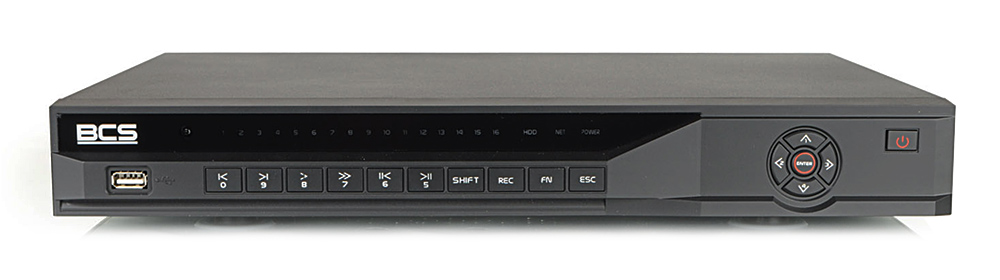
\includegraphics[width=0.8\linewidth]{gfx/bcs}}
\caption[Rejestrator BCS-NVT0802]{Rejestrator BCS-NVT0802.}
\label{fig:bcs}
\end{figure}

Prace techniczne i koncepcyjne poprzedziło badanie rynku. Za pomocą porównywarek cenowych zacząłem oceniać i porównywać oferty systemów monitoringu z różnych zakresów cenowych i jakościowych. Przyznaję, że w najniższej półce cenowej odnalazłem oferty o akceptowalnych parametrach. Jako przykład zostanie podany system monitorowania bezprzewodowego Conrad 8103J \ref{fig:bcs}, kameraIR, odbiornik 4-kanałowy. Producent zachwala rozwiązanie jako idealne do indywidualnego monitoringu wideo. W opisie produktu odnajdujemy informację, że komunikacja odbywa się po drodze radiowej, istnieje możliwość oglądania obrazu na ekranie monitora, oraz automatyczne diody podczerwieni umożliwiają transmisję czarno-białego obrazu w nocy.  Koszt zestawu wynosi 275 PLN.  

\begin{figure}[bth]
\centering
{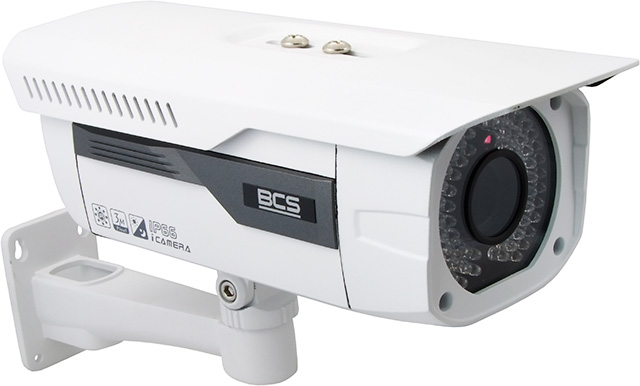
\includegraphics[width=0.6\linewidth]{gfx/bcsCam}}
\caption[ Kamera sieciowa BCS-TIP7300IR]{ Kamera sieciowa BCS-TIP7300IR.}
\label{fig:Chipscope}
\end{figure}

\begin{table}[b!]
%\myfloatalign
\caption[Conrad 8103J, kameraIR, odbiornik 4-kanałowy - dane i specyfikacja.]{Conrad 8103J, kameraIR, odbiornik 4-kanałowy - dane i specyfikacja.}
\begin{tabularx}{\textwidth}{|l|X|} 
 \hline
Dodatkowe światło IR & Tak \\ 
Komunikacja Analogowa, Radiowa Mikrofon &Tak \\
Napięcie robocze & 8 V/DC z zasilacza \\ 
Rodzaj kamery CCTV &  Bezprzewodowy system monitorujący \\
Rozdzielczość (TVL)& 720 x 480 p \\
Wymiary (odbiornik)& 24 x 78 x 107 mm \\  
Wymiary nadajnika & 26 x 35 mm \\ 
Zakres temperatury roboczej & od -10 do +50  C\\ 
Zasięg maksymalny & 100 m \\ \hline
\end{tabularx}  
\label{tab:compareAnalysers}
\end{table}

Z drugiej strony porównano rozbudowany system monitoringu IP: „Rejestrator BCS-NVR0802, 8 x Kamera BCS-TIP7300IR, Dysk 500GB, Akcesoria” firmy ivel electronics. Koszt zestawu 25 849,00 zł . W specyfikacji urządzania można odnaleźć bardzo wydajny sprzęt: 
Rejestrator BCS-NVR0802: 8 kanałowy sieciowy rejestrator cyfrowy z kompresją obrazu H.264, standard PAL. Nagrywanie do 8 kamer IP w D1 (25 kl/s), 720P (25 kl/s), 1080P (12 kl/s)



Prędkość zapisu rejestratora wynosi 200 klatek na sekundę (100 klatek w 1080P)
Wydajny procesor Dual-Core z systemem Embedded Linux, 8x Video, 8 x Audio, VGA, BNC, USB, HDMI, PTZ, RS485, Wyjścia/Wejścia alarmowe.
W rejestratorze można zamontować 2 dyski HDD SATA.
Możliwy podgląd przez internet na komputerze, smartfonie i tablecie. 

W zestawie jest też kamera sieciowa IP 3MPix FULL HD, 20 kl/s @3MPix (2048 x 1536), 25 kl/s @1080p. Przetwornik 1/2.8" SONY Progressive Scan CMOS. Obiektyw 8 - 16 mm/F1.6 CS Auto Iris, PoE, mechaniczny filtr podczerwieni. Zasięg podczerwieni 30 metrów. Hermetyczna  obudowa  klasy IP66 .

Po przeanalizowaniu dostępnych rozwiązań zaskakujący wniosek nasuwa się sam. Zauważamy sprzęt o bardzo dobrych parametrach, dostępny cenowo, ale niepraktyczny dla zwykłego użytkownika. Monitorując w dużej ilości zastosowań nie potrzebujemy nagrywać pełnometrażowego filmu z dużą dokładnością, który monitoruje obszar, w którym tak naprawdę niewiele się zmienia. Znacząca część zastosowań nie wymaga archiwizowania dużej ilości danych. Podgląd ze smartfona jest cennym dodatkiem aczkolwiek chcemy aby system sam informował o interesujących nas zdarzeniach i nie absorbował użytkownika w celu monitorowania obszaru. Konkluzją analizy dostępnych komercyjnych rozwiązań jest koncepcja zaprojektowania „Szybkiej, Inteligentnej kamery z interfejsem Ethernet”. Spośród istniejących rozwiązań kamera ma wyróżniać się właśnie na polu zastosowania. Tani wydajny sprzęt w połączeniu z algorytmami rozpoznawania obrazu możliwi opracowanie kamery bezkonkurencyjnej pod względem użyteczności, elastyczności zastosowania oraz pełnego wykorzystania potencjału sprzętowego.

\section{Przegląd dostępnych systemów wbudowanych}
Poniżej przedstawiono kilka z wielu dostępnych na rynku urządzeń, które mogą być zastosowane np. do rozwiązań typu „smart”.

Raspberry Pi 2 firmy Raspberry Pi Foundation jest minikomputerem wyposażonym w wydajną, 4-rdzeniową jednostkę SoC BCM 2836 firmy Broadcom. Posiada min.  złącze HDMI, 4 złącza USB i jedno Ethernet’owe. Ponadto kontroler kart SD, pozwala uruchomić system operacyjny z karty microSD. Płyta posiada także złącza dla dedykowanej kamery RaspiCam (sensor ov5xx) oraz złącze Display port, dla wyświetlacza. Cena : 175 zł

\begin{figure}[bth]
\centering
{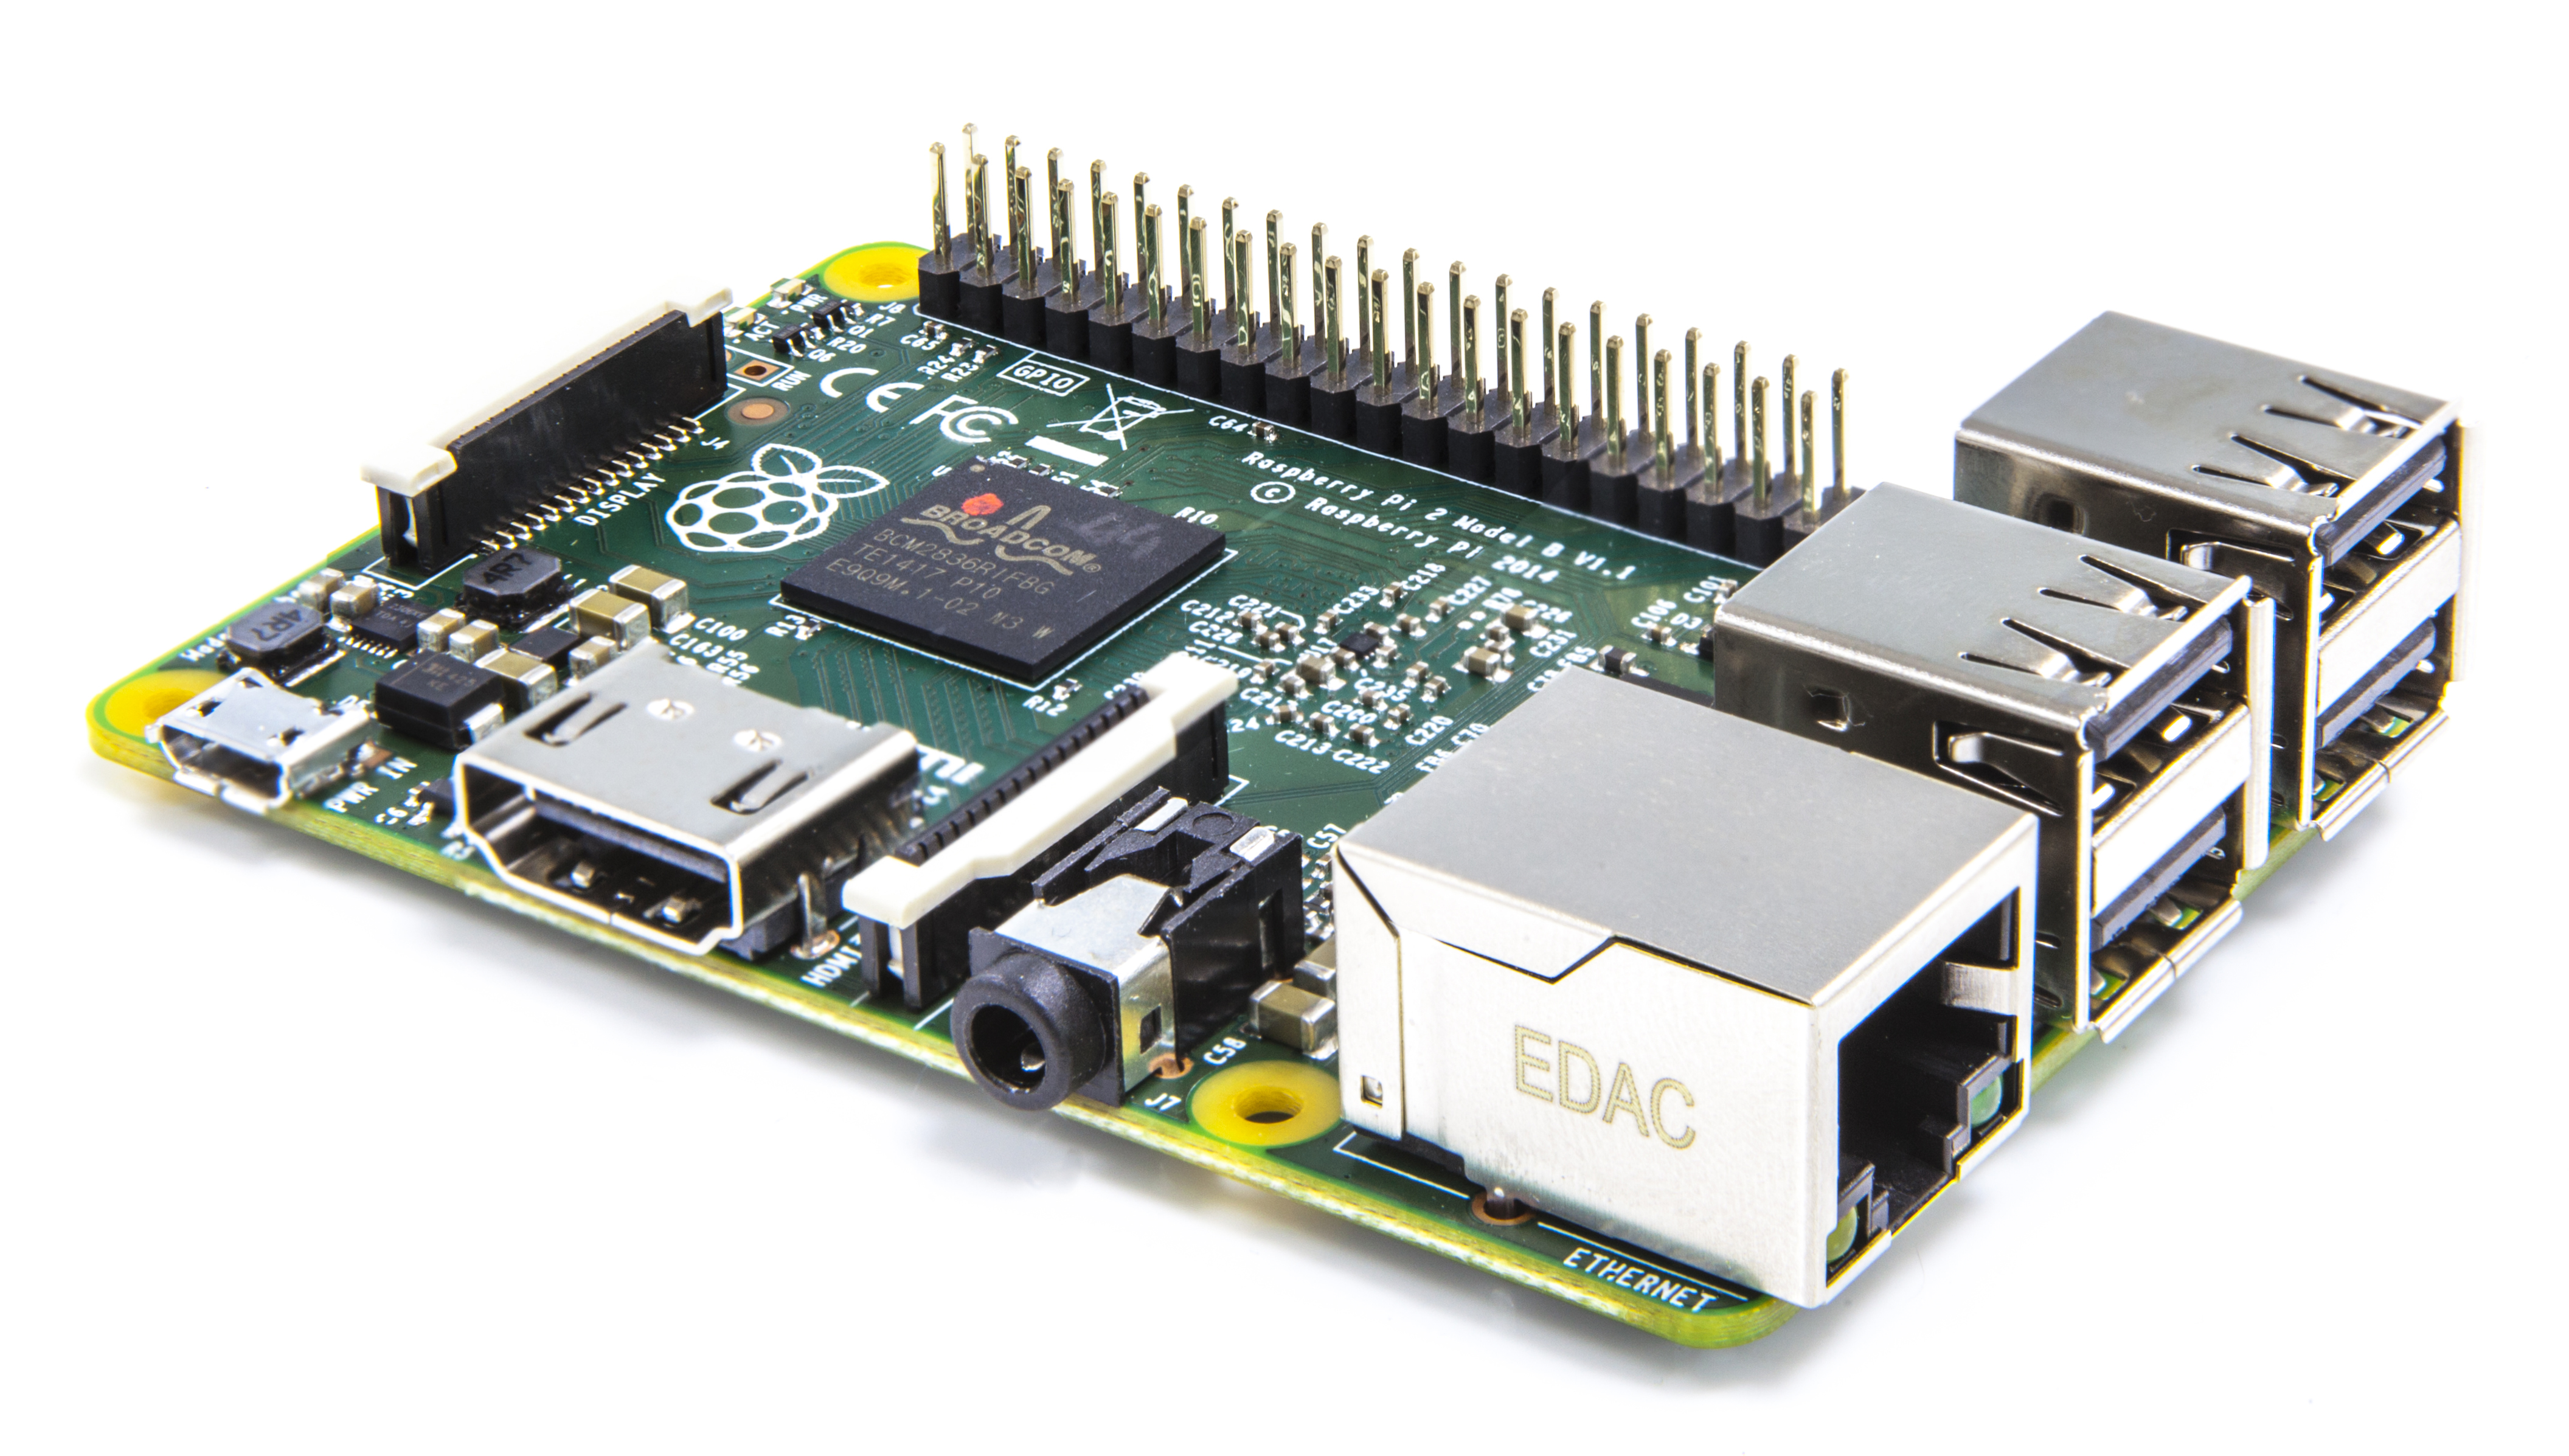
\includegraphics[width=0.8\linewidth]{gfx/rasp}}
\caption[Raspberry Pi w wersji 2]{Raspberry Pi w wersji 2}
\label{fig:Chipscope}
\end{figure}

BeagleBone Black Rev. C firmy BeagleBoard wyposażony w wydajny procesor Sitara AM335x firmy Texas Instruments taktowany zegarem 1GHz, 512 MB pamięci RAM i akcelerator grafiki 3D, a także złącza USB, HDMI i 92 porty GPIO. Cena: 249zł.

\begin{figure}[bth]
\centering
{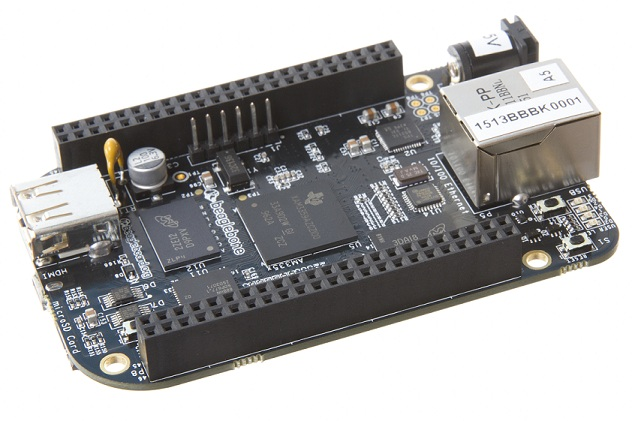
\includegraphics[width=0.8\linewidth]{gfx/beagle}}
\caption[BeagleBone Black Rev. C]{BeagleBone Black Rev. C}
\label{fig:Chipscope}
\end{figure}

OlinuXino Micro A13 firmy Olimex  z jednostką SoC Allwinner A13 i rdzeniem A13 Cortex A8 taktowanym zegarem 1GHz oraz jedostką GPU 3D Mali400 i 256 MB RAM stanowi tańszą alternatywę dla ww. urządzeń. Płyta posiada złącza USB, kontroler kart SD oraz wyjście VGA. Ponadto ma też osobne złącze dla wyświetlacza LCD i 40 portów GPIO. Cena: 35 EUR.

\begin{figure}[bth]
\centering
{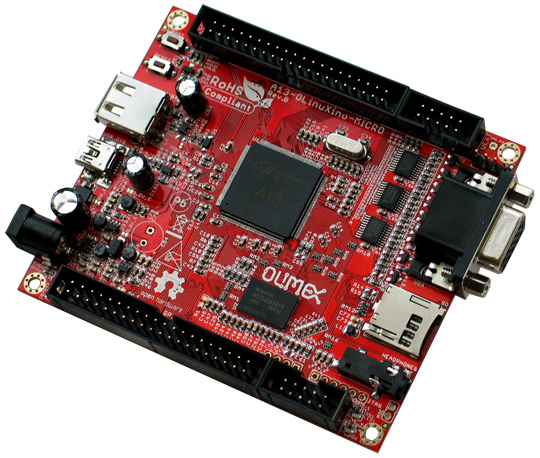
\includegraphics[width=0.6\linewidth]{gfx/olimex}}
\caption[OlinuXino Micro A13]{OlinuXino Micro A13}
\label{fig:Chipscope}
\end{figure}

Do zestawienia dodano rozwiązanie typowo z zastosowań przemysłowych: Wandboard Solo (model jednordzeniowy). Processor: Freescale i.MX6 Solo. Cores: Cortex-A9 Single core 
Graphic engine: Vivante GC 880 + Vivante GC 320. Memory: 512 MB DDR3. Warto wspomnieć o tym rozwiązaniu z powodu jego rosnącej popularności. Mały komputer jednopłytkowy wyróżnia solidne wykonanie, niezawodność oraz możliwość własnej adaptacji nakładek edm1 wykorzystującej standardowe złącze EDM. 

Do płytek nakładkowych typu edm (firmy Wandboard) lub rozwiązań SOM firmy olimex można opracować płytkę bazową, która będzie zinegrowana z kamerką i peryferiami komunikacji. Umożliwi to zmniejszenie rozmiaru, wykorzystanie tylko tych elementów, które są niezbędne. Zmniejszy to koszt projektu. Będziemy mieli również gwarancję, że jak zmieni się procesor będzie można wymienić płytkę nakładkową z procesorem (bez konieczności zmiany projektowej płytki bazowej).

Przyszłościowe koncepcyjne myślenie o rozwoju produktu skłoniło do wyboru dwóch rozwiązań, mniej popularnego tańszego układu firmy olimex i popularnych układów raspbery pi (z proc. BCM 2386). Oba wybrane zestawy demonstracyjne posiadają swoje odpowiedniki w płytach bazowych do rozwoju urządzeń tzw SOM (System on Module).

\begin{figure}[bth]
\centering
{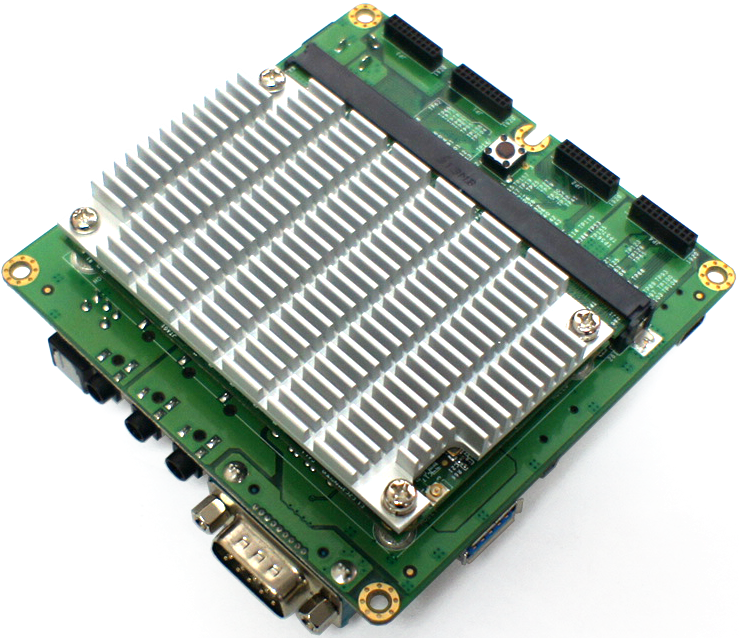
\includegraphics[width=0.6\linewidth]{gfx/wand}}
\caption[Wandboard]{Wandboard Solo}
\label{fig:Chipscope}
\end{figure}


\begin{table}[b!]
%\myfloatalign
\caption[Porównanie specyfikacji dostępnych rozwiązań.]{Porównanie specyfikacji dostępnych rozwiązań.}
\begin{tabularx}{\textwidth}{|lXXXXXX|} 
 \midrule
Urządzenie        & Procesor &Pamięć RAM & GPU & Interfejs kamery CSI & Ethernet & Cena \\
 \midrule
Raspberry Pi2       &  BCM 2386 900MHz quad-core ARM Cortex-A7 CPU &  1GB DDR2 SDRAM   &                     VideoCore IV &     Tak     &    10/100M  &  175 PLN\\
Beagle Bone Black Rev. C & AM335x 1GHz ARM Cortex-A8 & 512MB DDR3 RAM & PowerVR SGX530 & Nie & 10/100M & 249 PLN \\
OlinuXino Micro A13 & Allwinner A13 ARM Cortex A8 @1GHz & 256MB DDR2 RAM & 3D Mali400 & Tak & Nie (dostępny moduł USB-Ethernet)& 140 PLN \\
Wandboard Solo & Freescale i.MX6 Solo. & 512 MB DDR3 & Vivante GC 880 + Vivante GC 320 & ?? POSZUKASZ SAM ??? & 10/100M & 79 USD \\
\bottomrule
\end{tabularx}  
\label{tab:compareAnalysers}
\end{table}
%------------------------------------------------


\section{Architektura systemu Linux}
Obecnie Linux w systemach embedded \_ jest jednym z najpopularniejszych systemów operacyjnych. Dzięki uniwersalności i elastyczności można go spotkać w wielu urządzeniach dostępnych na rynku, takich jak : smartfony, tablety, odtwarzacze etc. Ważnym zagadnieniem w pracy z systemami opartymi na jądrze Linux jest znajomość jego architektury, a także połączenie wiedzy z  jego działania, administracji, konfiguracji oraz programowania w środowisku systemowym. W podrozdziale tym scharakteryzowane zostały podstawowe elementy każdego systemu opartego na jądrze Linux.

\begin{figure}[bth]
\centering
{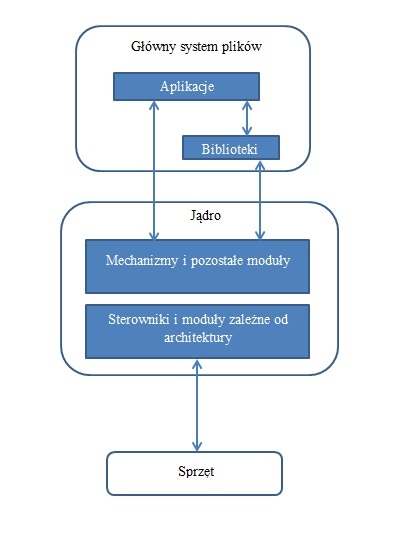
\includegraphics[width=0.7\linewidth]{sch/sch1}}
\caption[Architektura systemu Linux.]{Architektura systemu Linux.}
\label{fig:sch1}
\end{figure}

Jądro systemu – centralny element systemu operacyjnego, uprzywilejowany egzekutor zarządzający wszystkimi zasobami systemu. 

Moduły jądra – działają w uprzywilejowanym trybie; pozwalają na rozszerzanie funkcjonalności jądra bez ingerencji w kod źródłowy systemu.
Sterowniki – pośredniczą w komunikacji jądra ze sprzętem, oraz urządzeń wirtualnych (abstrakcyjnych)
Główny system plików – drzewo katalogów i plików

Biblioteki – używane przez niemal każdą aplikację; umożliwiają rozszerzenie funkcjonalności aplikacji działającej pod kontrolą systemu oraz stanowią interfejs do usług systemowych jądra.
Aplikacje – przenośne na poziomie kodu. Do podstawowych należą : powłoka, programy do operacji na plikach i katalogach, procesach, mechanizmach sieciowych, a także środowiska graficzne, kodery audio/wideo oraz wiele innych standardowych aplikacji.

\section{Dystrybucje systemu Linux}

Jako dystrybucję systemu Linux można określić kompletny system operacyjny, w skład którego oprócz samego jądra wchodzą dodatkowe usługi i aplikacje. To co odróżnia poszczególne dystrybucje, to jednolita organizacja plików konfiguracyjnych i mechanizm instalacji i zarządzania pakietami.
\begin{description}
\item Istnieje kilka kryteriów klasyfikacji dystrybucji:

\begin{itemize}[noitemsep]
\item Komercyjne lub niekomercyjne
\item Przeznaczone dla określonej grupy odbiorców : użytkowników zwykłych lub biznesowych
\item Wieloplatformowe, lub optymalizowane pod wybraną platformę sprzętową
\item Wyspecjalizowane lub ogólnego przeznaczenia
\item O określonym priorytecie np. przenośności czy bezpieczeństwa
\end{itemize}
\end{description}
\begin{description}
\item Wśród systemów wbudowanych opartych na platformie Raspberry można wyróżnić następujące dystrybucje:
	\begin{itemize}[noitemsep]
	\item Raspbian – najpopularniejsza dystrybucja, oparta na Debianie
	\item ArchLinux – pozwala w pełni dostosować system do wymagań użytkownika; pozbawiona GUI
	\item OpenELEC – dystrybucja typu Media Center
	\end{itemize}
\end{description}

W projekcie wykorzystana zostanie dystrybucja Raspbian .

\section{Konkurencyjne rozwiązania}

\begin{figure}[bth]
\centering
{
\includegraphics[width=0.3\linewidth]{sch/WE}}
\caption[Windows Embedded 7]{Windows Embedded 7}
\label{fig:sch1}
\end{figure}

Konkurencyjnym rozwiązaniem wchodzącym dynamicznie na rynek jest windows embedded.  Z każdą wersją obecnego systemu Windows udostępnia okrojoną wersję embedded. Rozwiązanie ma swoje zalety np. support techniczny, kompatybilność z aktualnymi desktopowymi systemami windows. Jako ciekawostkę można podać, że wymagania desktopowego systemu windows xp spełnia większość systemów wbudowanych, jak czyamy w wymaganiach systemu \footnote{https://support.microsoft.com/pl-pl/kb/314865}. Za wyborem linuxowego rozwiązania decydowało otwarte oprogramowanie, możliwość edycji ustawień systemowych z pozmiou kompilacji systemu. Pomijając indywidualne preferencje autora nie należy również zapominać, że systemy linux charakteryzują się bezpieczeństwem i jest to sprawdzone rozwiązanie dla systemów wbudowanych.

\section{Podsumowanie}
Na podstawie zestawienia popularnych systemów wbudowanych można stwierdzić, że każdy z nich oferuje różne konfiguracje i peryferia, co zmusza projektanta do optymalnego wyboru platformy sprzętowej pod kątem projektu. Analiza dostępnych urządzeń i dobranie optymalnego i niezawodnego rozwiązania stanowi ważny aspekt niniejszej pracy.
Najlepszy stosunek cena/jakość ma  Raspberry Pi 2. Czterordzeniowy procesor i 1GB pamięci RAM daje dużo większe możliwości względem konkurencyjnych produktów, co jest kluczowe przy  wymagających aplikacjach wykorzystujących przetwarzanie obrazu.
Jako dystrybucję systemu uruchamianą na płycie wybrano Raspbian.


	% Chapter cel pracy

\chapter{Cel i założenia pracy} % Chapter title

%\label{ch:name} % For referencing the chapter elsewhere, use \autoref{ch:name} 

 
Praca ma na celu zbadania możliwości wykonania projektu Szybkiej, Inteligentnej kamery z interfejsem Ethernet na systemie wbudowanym (ang. embedded system).
Kamerę stosować można będzie np. do monitorowania przestrzeni przemysłowej, a także w komunikacji miejskiej, czy też w zastosowaniach domowych. Docelowo użytkownikiem mają być osoby indywidualne, aczkolwiek system jest elastyczny, wobec czego łatwo można go zmodyfikować także pod kątem bardziej specjalistycznych zastosowań.
Projekt stanowi podstawę do realizacji dużo większego systemu – sieci kamer połączonych ze sobą, np. pod kontrolą serwera i umożliwiających realizację bardziej złożonych zadań, jak np. śledzenie trasy danej osoby, czy też kontrolowanie jednocześnie kilku obszarów w hali produkcyjnej.

\begin{description}
\item Założenia projektu :
	\begin{itemize}[noitemsep]
	\item Inteligencja dostosowana do wymogów monitoringu – zaimplementowana logika pozwala kamerze rozpoznać określone obiekty oraz wykonywać samodzielnie akcje, sterować układem zewnętrznym
	\item Maksymalizacja prędkości działania
\item Modularność – struktura oprogramowania ma być łatwa do rozbudowy i debugowania
\item Komunikacja z użytkownikiem.
		\end{itemize}
\end{description}

Do komunikacji z użytkownikiem wykorzystany zostanie serwer http, na którym będą umieszczane przez aplikację logi (zdjęcie osoby i data wykonania akcji). Natomiast sterowanie innymi urządzeniami zrealizowane jest poprzez wystawienie stanów HIGH/LOW na wyjściach portów GPIO.

\begin{description}
\item Na wykonanie projektu składa się:
\begin{itemize}[noitemsep]
\item Praca koncepcyjna
\item Konfiguracja systemu 
\item Połączenie podzespołów : płyty z układem sterowanym
\item Napisanie aplikacji uruchamianej na płycie
\item Skonfigurowanie serwera http i przygotowanie skryptu PHP/jQuery
\item Wykonanie testów działania projektu.
\end{itemize}
\end{description}
	\chapter{Koncepcja}

W rozdziale omówiona zostanie koncepcja i zasada działania inteligentnej kamery. 

\section{Maksymalizacja szybkości}
 
Szybkość działania kamery jest jednym z kluczowych założeń działania systemu. W zależności od przeznaczenia systemu może się znacznie różnić. W dziedzinach wyspecjalizowanych, takich jak robotyka, czy TODO
\begin{description}
\item Czynniki składające się na ogólną szybkość działania kamery:
	\begin{enumerate}[noitemsep]
	\item Przetwarzanie obrazu przez sensor oraz protokół komunikacyjny między sensorem, a płytą.
Według danych producenta czas potrzebny na wygenerowanie jednej klatki wynosi ok 1/90 s dla rozdzielczości strumienia 640x480. Protokół zastosowany w kamerze, to Camera Serial Interface wykorzystujący 2 linie danych umożliwiających maksymalną prędkość przesyłu na poziomie 2Gbps (1Gbps na linię).
\item Przetwarzanie obrazu przez sterownik obrazu (kompresja danych).
Czas ten jest uwarunkowany wydajnością akceleratora graficznego i  ze względu na wydajną jednostkę GPU VideoCore IV uznawany jest w projekcie za pomijalny.
\item Przetwarzanie danych przez aplikację.
Głównym czynnikiem mającym wpływ na ten czas jest algorytm zastosowany do detekcji twarzy. Dokładny jego opis znajduje się w rozdziale 3.6.1
\item Szybkość przesyłu danych przez interfejs Ethernet
Protokół Ethernet jest jednym z podstawowych interfejsów komunikacji urządzeń w lokalnych sieciach komputerowych. Zastosowana w płycie Raspberry Pi 2 wbudowana karta sieciowa wg informacji producenta umożliwia transfer danych z przepustowością 10 lub 100 Mb/s.
		\end{enumerate}
\end{description}

Ważnym aspektem są czas odpowiedzi systemu dla każdej z ww. operacji oraz ogólne czasy odpowiednio między wykryciem twarzy a : \\
-akcją sprzętową (np. otwarciem drzwi, włączeniem alarmu)\\
-umieszczeniem logu na serwerze.\\
W projekcie przyjęto założenie, że w celu poprawy skuteczności detekcji obiektu minimalny czas między zdarzeniem wykrycia obiektu określony będzie przez użytkownika. Rozdział  4. aspekt ten opisuje dokładniej.

\section{Inteligencja dostosowana do wymogów monitoringu}
Inteligentny system monitorujący wymaga, aby oprócz dostarczania obrazu dokonać także jego przetworzenia – tj. za pomocą odpowiednich algorytmów dokonać detekcji żądanych obiektów.
Podrozdział 3.6.1 traktuje szczegółowo o tym zagadnieniu.

\section{Modularność }

\begin{description}
\item Struktura modularna pozwala zapewnić dużą kontrolę przy projektowaniu i debugowaniu działania aplikacji. Aplikacja jest pisana zgodnie z techniką programowania obiektowo orientowanego (w skrócie OO), wyróżnić można kolejne kroki :
\begin{enumerate}[noitemsep]
\item Rozpoznanie problemu. \\%enter
Przeprowadzona została analiza funkcjonalności systemu i wymagań, zgodnie z założeniami z rozdziału 3.1.
\item Projektowanie programu. \\
Na ten etap składa się : zidentyfikowanie zachowań systemu i obiektów w nim występujących, a następnie określenie ich hierarchii ( dziedziczenie ) i sekwencji działania.



Obiekty występujące w systemie to :
\begin{itemize}[noitemsep]
\item Module – bazowa klasa abstrakcyjna
\item Object Detect – klasa implementująca detekcję obiektów
\item Worker – klasa odpowiedzialna za wszelkiego rodzaju akcje
\item Logger – klasa implementująca mechanizm generowania logów. Współpracuje bezpośrednio z Object Detect
\item Controller – główna klasa zarządzająca pozostałymi, implementuje „logikę” kamery.
\end{itemize}

Do konkretnych zachowań można zaliczyć : detekcję obiektów, wykonanie akcji (sterowanie portami GPIO), stworzenie pliku logów. Każda z wymienionych klas dziedziczy po Module.
Sekwencja działania jest zdefiniowana następująco :
\begin{enumerate}[noitemsep]
\item Object Detect po wykryciu twarzy, wysyła sygnał do Controllera
\item Controller ustawia flagę detected=true, odczekuje ustalony przez użytkownika czas \textbf{latency }
\item Jeśli po upływie \textbf{latency} Controller otrzyma ponownie sygnał, to zleca modułowi Worker i Logger pracę - wykonanie akcji sprzętowej i wygenerowanie pliku z logiem.
\item Po wykonaniu pracy Worker wysyła do Controllera sygnał
\item Po odebraniu sygnału od Worker’a Controller zatrzymuje pracę modułu Object Detect
\item Po wykryciu zamkniętych drzwi Worker wysyła sygnał do Controllera
\item Odebranie sygnału od Workera powoduje wznowienie pracy Object Detect
\end{enumerate}
\item Implementacja: \\
Implementacja komunikacji między obiektami zrealizowana jest z wykorzystaniem mechanizmu sygnałów biblioteki Boost. Daje to możliwość przekazania sterowania danemu obiektowi poprzez wywołanie funkcji obiektu zlecanego - zbindowanej w slocie wraz z przekazanym argumentem określonego typu.
\item Testowanie: \\
Ważnym aspektem poprawnej pracy systemu są testy. System musi spełniać nie tylko warunek poprawnego działania, ale też spełniać wymagania czasowe. Rozbieżności takie mogą w konsekwencji prowadzić do trudnych do wykrycia awarii, niekoniecznie urządzenia kamery ale np. urządzenia sterowanego, czy też powodować zakłamania w wynikach pracy kamery.
Argumentem dla wyboru techniki OO jest fakt, iż system w przyszłości może realizować inne zadania/warunki, w konsekwencji aplikacja będzie potencjalnie modyfikowana i sukcesywnie rozbudowywana.
\end{enumerate}
\end{description}

\section{Interface użytkownika}
Jako interfejs użytkownika służy serwer http – Apache 2. Na podstawie dostarczonych od modułu Logger  zdjęć generuje odpowiednie wpisy i umieszcza je na stronie WWW. Za generację logów po stronie serwera odpowiedzialne są skrypty napisane z wykorzystaniem technologii PHP i jQuery.

Dane takie jak data, godzina są zawarte w nazwie plików, natomiast zostaną wyodrębnione przez ww. skrypty. Strona WWW odświeżana jest automatycznie  co 1s.  Szczegółowy opis działania skryptów opisany jest w podrozdziale 3.6.3.

\section{Funkcje systemu}

%Funkcje systemu :
\begin{itemize}[noitemsep]
\item Detekcja obiektów \\
Obiekty te mogą być w zasadzie dowolnego typu. Detekcja opiera się na wytrenowaniu algorytmu dlatego mogą to być zarówno obiekty rzeczywiste, takie jak: twarze ludzkie, litery, pojazdy itp., oraz specyficzne wzory pozwalające identyfikować jednoznacznie żądane obiekty.

\item Sterowanie modułem zewnętrznym \\
W zależności od wymagań mogą to być: manipulatory robotów, sterowniki bram, napędy, czujniki, a także inne aplikacje, które oczekują na informacje od kamery ( np. ilość obiektów i ich czasy poruszania się, czy też orientacja w przestrzeni).

\item Logowanie zdarzeń na serwerze http \\
Dzięki interfejsowi Ethernet możliwa jest komunikacja systemu z użytkownikiem. Np. umieszczanie na serwerze logów, lub danych przetworzonych przez urządzenie w bazie danych. 

\item GUI \\ 
Dodatkową funkcjonalnością przewidywaną przy dalszej rozbudowie systemu jest graficzny interfejs użytkownika GUI (ang. Graphic User Interface), pozwalający na szybszą i  bardziej intuicyjną interakcję użytkownika z systemem.

\item Sterowanie zewnętrznymi akcjami \\
W projekcie kamera łączy role systemu monitoringu i sterownika drzwi:  ma za zadanie wykryć twarze osób, które pojawią się przed drzwiami, a następnie je otworzyć. Kolejnym krokiem jest umieszczenie  na serwerze logu w postaci : zdjęcia danej osoby oraz daty i godziny pojawienia się. Dostęp do logów będzie możliwy dla każdego użytkownika posiadającego urządzenie posiadające przeglądarkę stron WWW ( czyli smartfony, tablety, komputery itd.) i będące w obrębie sieci, w której pracuje kamera.
Ogólna idea zastosowania kamery jest zilustrowana na rysunku 3.1.
\end{itemize}

\begin{figure}[bth]
\centering
{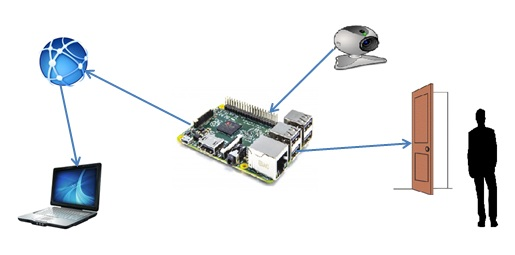
\includegraphics[width=1\linewidth]{sch/Koncepcja_ogolna_projektu}}
\caption[Koncepcja ogólna projektu]{Koncepcja ogólna projektu}
\label{fig:sch2}
\end{figure}

\section{Szczegółowe omówienie funkcji}
\subsection{Detekcja obiektów}
Do realizacji detekcji obiektów wykorzystana zostanie biblioteka OpenCV (Open Computer Vision). Bibliotekę tę cechuje wieloplatformowość, kilka interfejsów programistycznych, modularna struktura oraz wiele algorytmów z zakresu wizji komputerowej i uczenia maszynowego. 

W projekcie użyty został interfejs C++, natomiast platformą docelową jest Linux w dystrybucji Raspbian.

Detekcja obiektów jest zaawansowanym zagadnieniem wizji komputerowej. Biblioteka OpenCV dostarcza wiele funkcji umożliwiających łatwe użycie algorytmów. Poniżej zamieszczony jest opis działania  algorytmu detekcji obiektów Viola-Jones.
 
\paragraph{Cechy algorytmu Haara.} Główną ideą działania algorytmu jest wykorzystanie przesuwnego, skalowalnego okna, które posiada tzw.  cechy Haara (ang. Haar features). 

Cechy te nakładane są na dany obraz w celu określenia przynależności danego obszaru do klasy obiektów poszukiwanych. Dla każdej cechy obliczana jest różnica sumy wartości pikseli znajdujących się na obszarach białych i czarnych.

\begin{figure}[bth]
\centering
{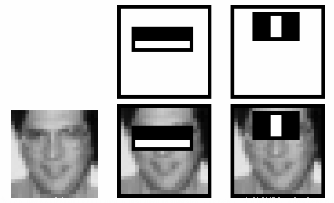
\includegraphics[height=0.35\linewidth]{sch/haar}}
{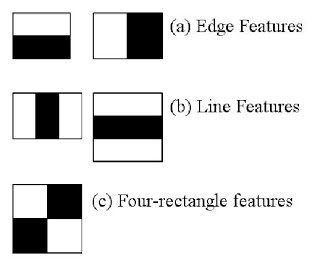
\includegraphics[height=0.35\linewidth]{sch/haar_features}} \\
\caption[ Cechy Haara i wykorzystanie cech Haara do detekcji twarzy.]{Cechy Haara i wykorzystanie cech Haara do detekcji twarzy.}
\label{fig:sch2}
\end{figure}

Uwzględniając wszystkie możliwe wymiary i położenia dla okna przesuwnego np. o wymiarach 24x24, liczba cech wynosi ponad 160 000. Ograniczone zasoby sprzętowe standardowych komputerów klasy PC, a tym bardziej systemów wbudowanych nie pozwalają na wykonanie tej skali obliczeń w sensownym czasie. Dlatego podstawową ideą jest wyeliminowanie ze zbioru cech, tych które są nieistotne w procesie detekcji. Tutaj z pomocą przychodzą obrazy całkowe(ang. Integral images) i algorytm AdaBoost (Adaptive Boosting).

\paragraph{Obrazy całkowe}
Pozwalają one na szybkie i efektywne obliczanie sumy wartości pixeli w określonym obszarze cechy.

Metoda ta wykorzystuje zależność, która pozwala obliczyć wartość sumy pixeli z obszaru ograniczonego przez zaledwie cztery punkty A=(x0,y0),B=(x1,y0),C=(x0,y1),D=(x1,y1) 

$$ \sum_{\binom{x0<x<x1}{y0<y<y1}} i(x,y) = I(D) + I(A) -I(B) - I(C)$$
gdzie:
$$ I(x,y) = \sum_{\binom{x'<x}{y'<y}}$$

Co zilustrowano na rysunku \ref{fig:sch2}.
\begin{figure}[bth]
\centering
{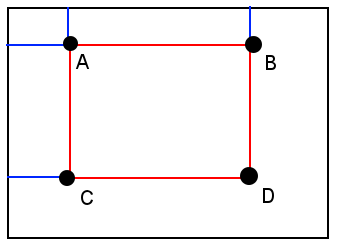
\includegraphics[height=0.35\linewidth]{sch/pxel}}
\caption[ Obliczanie sumy wartości pixeli fragmentu obrazu]{Obliczanie sumy wartości pixeli fragmentu obrazu.}
\label{fig:sch2}
\end{figure}




\paragraph{Algorytm AdaBoost} opracowany i zaprezentowany w 1997 r. przez Yoava Freunda i Roberta Schapire jest jednym z wielu realizujących tzw. boosting. W wyniku procesu uczenia algorytmu otrzymujemy silny klasyfikator binarny, który składa się ze słabszych klasyfikatorów z odpowiednimi wagami. Klasyfikator taki daje nam jednoznaczną informację czy dany obiekt należy do klasy poszukiwanych, czy też nie. Budowany jest w procesie uczenia, gdzie na wejście podaje się tzw. zestaw treningowy (ang. training set), a na wyjściu otrzymujemy gotowy klasyfikator zdolny do pracy z nowym zbiorem danych.
Klasyfikator słaby, to taki, którego błąd klasyfikacji jest mniejszy niż 0.5, czyli lepszy niż zwykłe zgadywanie.

Opis algorytmu:
%Algorytm AdaBoost
Wejście: zbiór przykładowych obrazów $(x_1,y_1),..,(x_n,y_n)$, gdzie $y_i=0,1$ dla odpowiednio negatywnych i pozytywnych próbek.
Wyjście: silny klasyfikator $H(x)$.
Kroki algorytmu :
\begin{enumerate}
\item Dla każdego z k elementów zestawu trenującego T  przypisz identyczną wagę początkową.
$$W^1(i)= \frac{1}{k}  , i = \{1,...,k\} $$
Liczba iteracji wynosi $N$.
\item Dla $n=1,…,N$: 
Wybierz słaby klasyfikator o najmniejszym błędzie $\epsilon_n$
	$$\epsilon_n = \sum_i W_i |h_n(x_i)-y_i	| $$
\item Oblicz nową wagę 
$$\alpha_n = \frac{1}{2} ln \frac{1-\epsilon_n}{\epsilon_n}$$  
\item Dla poprawnie sklasyfikowanych przykładów trenujących xi wagi są uaktualniane na podstawie zależności:
$$W_{n+1} = \frac{W_n(i)exp(-\alpha n)}{z}$$
Dla niepoprawnie sklasyfikowanych przykładów :
$$W_{n+1} = \frac{W_n(i)exp(\alpha n)}{z}$$
gdzie Z- stały czynnik normalizujący.
 
\item Klasyfikator końcowy:
 $$H(x) =\begin{cases}1 \sum^N_{n=1} \alpha_n h_n(x) \geq \frac{1}{2} \sum^N_{n=1} \alpha \\
 0 \end{cases} $$
\end{enumerate} 

Podsumowując AdaBoost wykorzystuje te cechy, które są w stanie wykryć samodzielnie więcej niż połowe przypadków. Poprzez zmniejszanie wag cech poprawnie wykrywających obiekty i zwiększanie wag  cech, które sklasyfikowały obiekty błędnie, algorytm	 potrafi „skupić się” na trudnych przypadkach.	
Klasyfikator zaproponowany przez autorów biblioteki OpenCV zawiera po wytrenowaniu około 6000 cech. Jest to ogromna redukcja względem wspomnianych 160 000,  jednakże wciąż zbyt dużo, aby zapewnić detekcję obiektu w krótkim czasie. Rozwiązaniem jest kaskada klasyfikatorów.
\paragraph{Kaskada klasyfikatorów}

Większość z obszaru analizowanych obrazów nie zawiera twarzy. Stąd wyszedł pomysł,  aby ocenić czy obszar może zawierać twarz już na samym początku. Jeśli nie, odrzucić ten region, a skupić się na tych, które faktycznie mogą zawierać twarz. Taki zabieg pozwala oszczędzić mnóstwo czasu i zasobów sprzętowych.
Zamiast sprawdzać wszystkie 6000 cech autorzy proponują podzielić proces detekcji na wiele etapów. W każdym z etapów są zgrupowane określone cechy nakładane jedna po drugiej, przy czym ilość cech sprawdzanych w kolejnych etapach rośnie. Jeśli obraz nie przejdzie początkowych etapów jest odrzucany i sprawdzany jest kolejny. Natomiast jeśli przejdzie wszystkie etapy – klasyfikowany jest jako twarz. Zasadę działania kaskady ilustruje rysunek \ref{fig:kaskada}.

\begin{figure}[bth]
\centering
{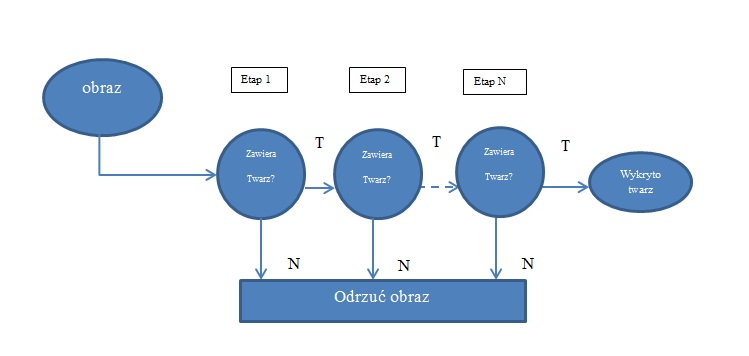
\includegraphics[width=1\linewidth]{sch/kaskada}}
\caption[Kaskada klasyfikatorów dla N etapów.]{Kaskada klasyfikatorów dla N etapów.}
\label{fig:kaskada}
\end{figure}

Biblioteka OpenCV w pakiecie zawiera także narzędzia, które pozwalają samemu wytrenować klasyfikator zdolny do rozpoznania dowolnych obiektów. Aby jednak wytrenować dość silny klasyfikator potrzeba dużej ilości pozytywnych i negatywnych przykładów. Stąd też zdecydowano się użyć dostarczonych w pakiecie biblioteki gotowych klasyfikatorów. Proces trenowania przedstawiony jest na schemacie \ref{fig:trening}. W wyniku działania narzędzia HaarTraining otrzymujemy plik XML ze zdefiniowanym klasyfikatorem, gotowym do użycia w aplikacji.

\begin{figure}[bth]
\centering
{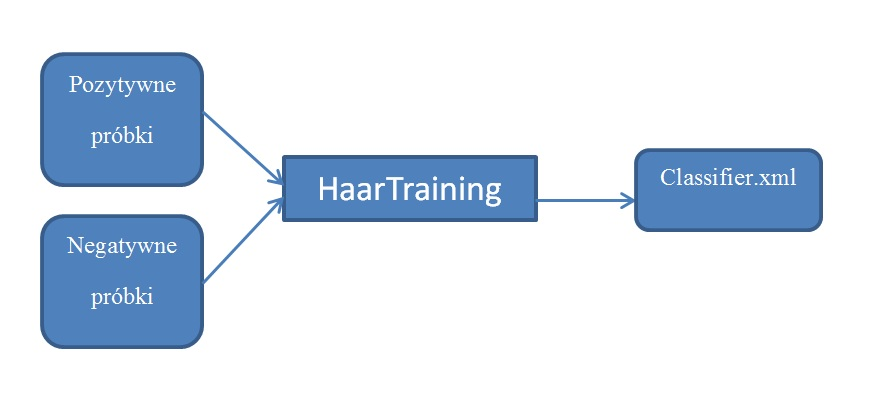
\includegraphics[width=1\linewidth]{sch/trening}}
\caption[Schemat trenowania klasyfikatora]{Schemat trenowania klasyfikatora}
\label{fig:trening}
\end{figure}

\subsection{ Sterowanie urządzeniem zewnętrznym}
Sterowanie urządzeniami zewnętrznymi zrealizowane jest przez programowe wystawianie stanów logicznych na portach GPIO płyty. Pozwala to po zestawieniu z układem sterowanym na kontrolę urządzeniem. W projekcie znajduje się implementacja, która pozwala na zaadaptowanie kamery do sterowania urządzeniem zewnętrznym. Sygnały cyfrowe można zastosować do dowolnego przeznaczenia np. włączenie alarmu, światła, klimatyzacji, powitania gościa...

 \begin{figure}[bth]
\centering
{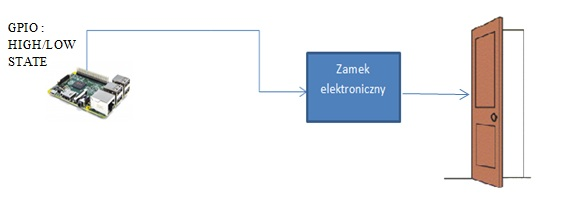
\includegraphics[width=1\linewidth]{sch/sterowanie}}
\caption[Koncepcja sterowania urządzeniem zewnętrznym]{Koncepcja sterowania urządzeniem zewnętrznym}
\label{fig:sterownie}
\end{figure}

\subsection{ Logowanie zdarzeń na serwerze HTTP}
Interfejs Ethernet zapewnia możliwość interakcji kamery z użytkownikiem.  Jej realizacja opiera się o serwer http, który  będzie wykonywał  skrypt napisany w technologii PHP i jQuery i wynik działania umieszczał na stronie internetowej.
Efektem czego użytkownik będzie mógł połączyć się z serwerem z dowolnego urządzenia, które posiada przeglądarkę stron WWW.  
\paragraph{Serwer http.}
Jako serwer wykorzystano Apache 2 – popularny, darmowy serwer http współpracujący z różnymi językami programowania oraz ze wsparciem dla baz danych – MySQL, PHP etc.
Współpracuje z systemami Linux, Windows i Mac OS. W projekcie uruchamiany jest na Linuxie.
 
 
\begin{figure}[bth]
\centering
{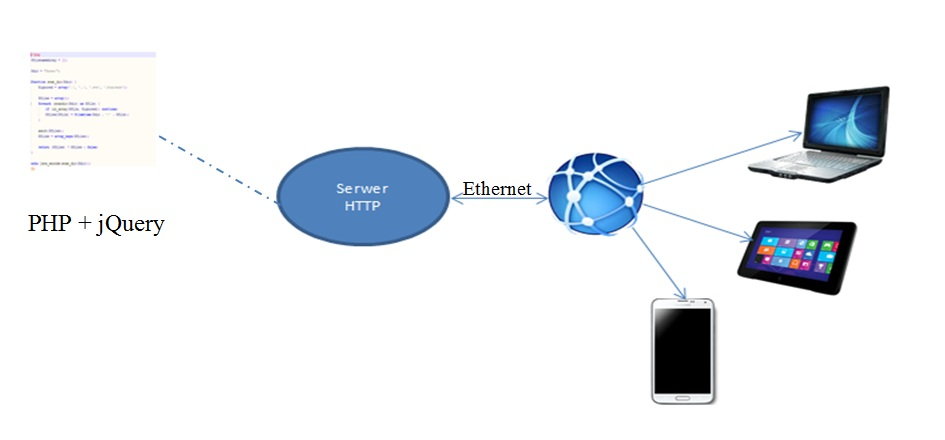
\includegraphics[width=1\linewidth]{sch/interface_komunikacji}}
\caption[Koncepcja interfejsu komunikacji z użytkownikiem]{Koncepcja interfejsu komunikacji z użytkownikiem}
\label{fig:komunikacja}
\end{figure}







	% Chapter IMPLEMENTACJA

\chapter{Realizacja} % Chapter title

Rozdział ten przedstawia opis szczegółowy koncepcji przedstawionych w rozdziale 3.

\section{Oprogramowanie}
\subsection{Narzędzia i środowisko pracy}
Jako środowisko robocze wykorzystano system Ubuntu 14.04. Do stworzenia aplikacji użyte zostało środowisko programistyczne Eclipse Kepler. Dzięki wielu wtyczkom dostępnym do tego IDE (ang. Integrated Development Environment), możliwa była min. wygodna współpraca z systemem kontroli wersji GIT. System kontroli wersji pozwolił na bezpieczne rozwijanie projektu, wraz z możliwością śledzenia istotnych zmian.

\begin{description}
\item Aby zapewnić poprawne działanie zarówno serwera HTTP, jak i kamery niezbędne są:
	\begin{itemize}[noitemsep]
	\item Sterownik UV4L - User-space Video for Linux autorstwa Luci Risolii. Jest to pakiet modułów przeznaczony dla rzeczywistych i wirtualnych urządzeń video  działający w przestrzeni użytkownika, kompatybilny z oficjalnym frameworkiem Video4Linux2 (Video for Linux 2). Moduł uv4l ładuje z poziomu linii komend wybrany sterownik i tworzy węzeł urządzenia video w katalogu /dev głównego systemu plików. Taki interfejs komunikacji z urządzeniem jest popularny w bibliotekach wykorzystujących strumienie video.\\
\begin{description}
\item Do niektórych cech pakietu należą : \\
\begin{itemize}[noitemsep]
\item Kompatybilność z Video4Linux 2 API
\item Dzięki pracy modułów w przestrzeni użytkownika, system (jądro) nie jest narażone na niestabilność
\item Możliwość dodania kilku urządzeń (każde z nich obsługiwane przez oddzielny proces)
\item Nie wymaga zewnętrznych bibliotek i pakietów
\end{itemize}
\end{description}
\begin{description}
\item W pakiecie dostępne są min. moduły:
\begin{itemize}[noitemsep]
\item UV4L core module - główny moduł 
\item Raspicam - moduł dla dedykowanej kamery Raspicam (sensor OV5647)
\item HTTP Streaming Server - sterownik przeznaczony do streamingu video z wykorzystaniem protokołu HTTP\\ 

\end{itemize}
\end{description}
W pracy wykorzystywane są dwa pierwsze, jednak wykorzystanie ostatniego z wymienionych daje możliwości rozszerzenia funkcjonalności kamery.\\
Obsługa pakietu z poziomu linii komend jest następująca:\\
uv4l $--$driver [moduł] $--$video\_nr [numer] $--$encoding [kodowanie] $--$width [szerokość] $--$height [wysokość] \\
Przykładowe wywołanie sterownika uv4l $--$driver raspicam --video\_nr 0 $--$encoding yuv420 $--$width 640 $--$height 480\\
Uruchomi moduł raspicam, który zarejestruje urządzenie pod węzłem /dev/video0 z kodowaniem strumienia YUV420 i rozdzielczością 640x480.\\
	\item Serwer HTTP Apache 2
		\end{itemize}
\end{description}


\subsection{Algorytm}
Działanie aplikacji opiera się o główny algorytm, który zaprezentowany jest na rysunku\ref{fig:algorytm}. Poniżej znajduje się jego opis :\\
\begin{enumerate}
\item Po starcie programu następuje jego konfiguracja - tworzony jest moduł\textbf{ Controllera} oraz moduły robocze. W zależności od tego, czy użytkownik podał argumenty wejściowe (rozdzielczość strumienia, czas latencji), \textbf{Controller} przekazuje je do modułu\textbf{ Object\_detection}, albo inicjuje wartościami domyślnymi (szerokość  = 320, wysokość = 240, latencja = 0). Oprócz tych parametrów ustawiane są wewnętrzne flagi niezbędne do poprawnego działania modułów. Są to odpowiednio flagi \textbf{detected} - ustawiana wstępnie na false oraz\textbf{ obj\_d\_en }- ustawiana wstępnie na true. Flaga \textbf{ obj\_d\_en } (object detect enable) odpowiada za zezwolenie modułowi wykrywania obiektów na pracę. W tej realizacji projektu ma stałą wartość - true, jednak na potrzeby realizacji innych koncepcji może zostać stworzona implementacja, gdzie flaga ta jest modyfikowana przez inne moduły lub wątki przesyłające sygnał do Controllera.\\
\item Sprawdzenie flagi \textbf{ obj\_d\_en}. Jeśli jej wartość jest prawdziwa przejdź do kroku 3. W przeciwnym przypadku przejdź do 2.\\
\item Do pracy rusza moduł \textbf{ Object\_detection}, a konkretnie funkcja robocza \textbf{work()}.
Jeśli zostanie wykryty obiekt, to moduł ten wysyła sygnał \textbf{Controllerowi}, przekazując mu tym samym sterowanie.\\
\item \textbf{Controller} bada czy wartość flagi \textbf{detected} jest prawdziwa. Jeśli nie, to wątek główny usypiany jest na okres latencji (argument \textbf{latency} podany przez użytkownika - czas w ms), \textbf{detected} ustawiana jest na true i następuje powrót do kroku 2. Jeśli tak, to następuje przejście do kroku 5.\\
\item Do pracy ruszają moduły \textbf{ Worker i Logger}. Flaga \textbf{detected }ustawiana jest na false. Następuje przejście do kroku 2.\\
Parametr \textbf{latency} zastosowany jest w celu walidacji obiektu detekowanego. Aby kamera nie logowała przypadkowo przechodzących osób lub błędnie sklasyfikowanych klatek strumienia video - poddawana jest dwukrotnej analizie. Po czasie ustalonym przez użytkownika (teoretycznie w zakresie od 0 do nieskończoności) Daje to niemal stuprocentową pewność poprawnej detekcji obiektu, jednakże kosztem wzrostu czasu odpowiedzi układu. Parametr ten jest opcjonalny i pozwala użytkownikowi samodzielnie skalibrować kamerę.
\end{enumerate}
\begin{figure}[bth]
\centering
{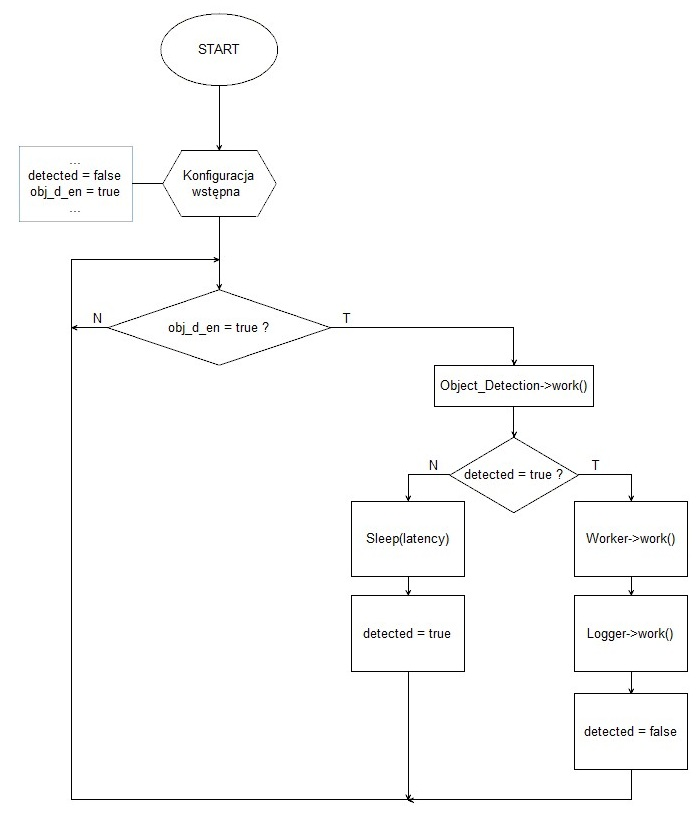
\includegraphics[width=1\linewidth]{sch/algorytm}}
\caption[Algorytm główny aplikacji.]{Algorytm główny aplikacji.}
\label{fig:algorytm}
\end{figure}
\subsection{Aplikacja}
Aby zapewnić elastyczność aplikacji i łatwość rozbudowy oraz debugowania zdecydowano się na modularną strukturę. Wyróżnić można w niej moduł odpowiedzialny za „logikę” – Controller oraz moduły wykonujące zadania – Object Detection, Worker, Logger.
Ważnym aspektem działania aplikacji jest komunikacja między modułami. W projekcie wykorzystano mechanizm sygnałów biblioteki Boost.
\begin{figure}[bth]
\centering
{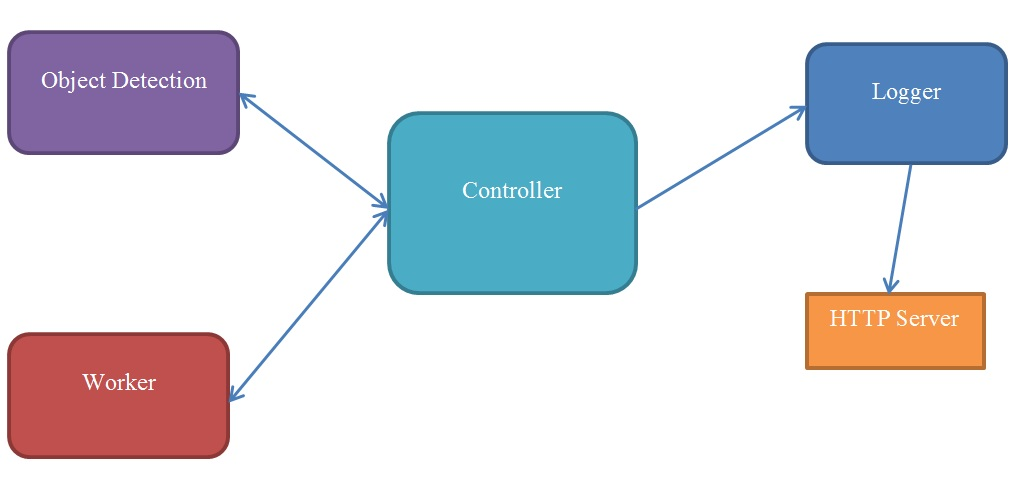
\includegraphics[width=1\linewidth]{sch/kooperacja_obiektow}}
\caption[Diagram współpracy obiektów]{Diagram współpracy obiektów.}
\label{fig:koooperacja}
\end{figure}

\paragraph{Controller} jest odpowiedzialny za przetwarzanie otrzymanych od innych modułów sygnałów i zlecanie im wykonania odpowiednich zadań. Po otrzymaniu sygnału od modułu Object Detect, Controller z wykorzystaniem mechanizmu sygnałów biblioteki Boost zleca modułowi Worker wykonanie akcji, zaś modułowi Logger  przygotowanie pliku logu, który zostanie przetworzony następnie przez serwer HTTP.
Moduł ten odbiera też sygnał zwrotny od Worker’a, potwierdzający wykonanie akcji i pozwala wznowić pracę modułu Object Detect.


\begin{lstlisting}[caption = {Klasa Controller.}, label=Controller, language=C++]
class Controller{
public:
	typedef boost::signals::connection conn;
	short int cam_w,cam_h,latency;
	boost::signal <bool(void *wsk)>SigC;
	bool detected;

	Module * modules[3];
	bool logicUnit(int nr,void* wsk);
		Controller(int w=320,int h=240,int l=2000);
		~Controller();
	
	private:
		conn c_obd;
		conn c_wor;
		conn c_log;
	};     
\end{lstlisting}


\begin{figure}[bth]
\centering
{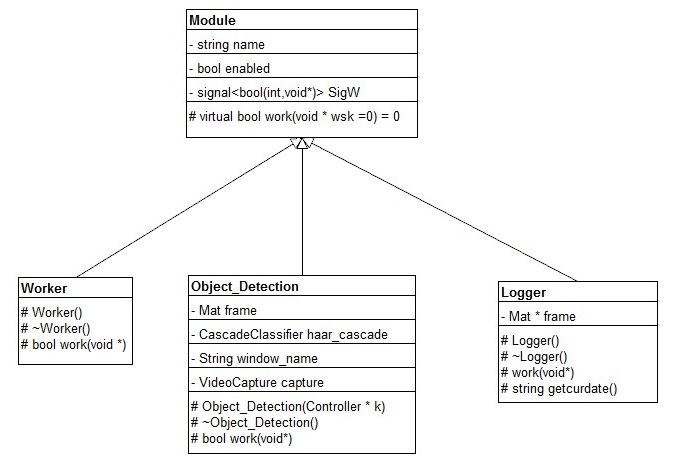
\includegraphics[width=1\linewidth]{sch/diagram_klas}}
\caption[Diagram klas roboczych]{Diagram klas roboczych.}
\label{fig:dziedziczenie}
\end{figure}
Na schemacie \ref{fig:dziedziczenie} zaprezentowana jest implementacja klas roboczych. Wszystkie moduły robocze dziedziczą po abstrakcyjnej klasie Module. Dzięki temu możliwa jest łatwa kontrola i dalsza rozbudowa aplikacji. Implementacja ta jest szczególnie przydatna przy pracy w zespole. Dzięki niej programista wykorzystujący moduł napisany przez innego członka zespołu nie musi znać szczegółowej implementacji - wystarczy, że zna ogólny interfejs i specyfikację modułu (w szczególności argumenty jakie powinien przekazać modułowi).

\paragraph{Object\_Detection} ma za zadanie wykryć obiekty ze strumienia video (dostarczanego przez kamerę podłączoną do płyty. Obiektami założonymi w projekcie są twarze ludzkie, jednak aplikacja jest pod tym względem elastyczna tj. wystarczy wytrenować klasyfikator dowolnego obiektu (narzędzie HaarTraining dostarczone w pakiecie z biblioteką OpenCV) i dołączyć  wygenerowany plik XML. Po wykryciu twarzy wysyłany jest sygnał do Controllera wraz ze wskaźnikiem do struktury frame z wyodrębnionymi twarzami z klatki.

\begin{figure}[bth]
\centering
{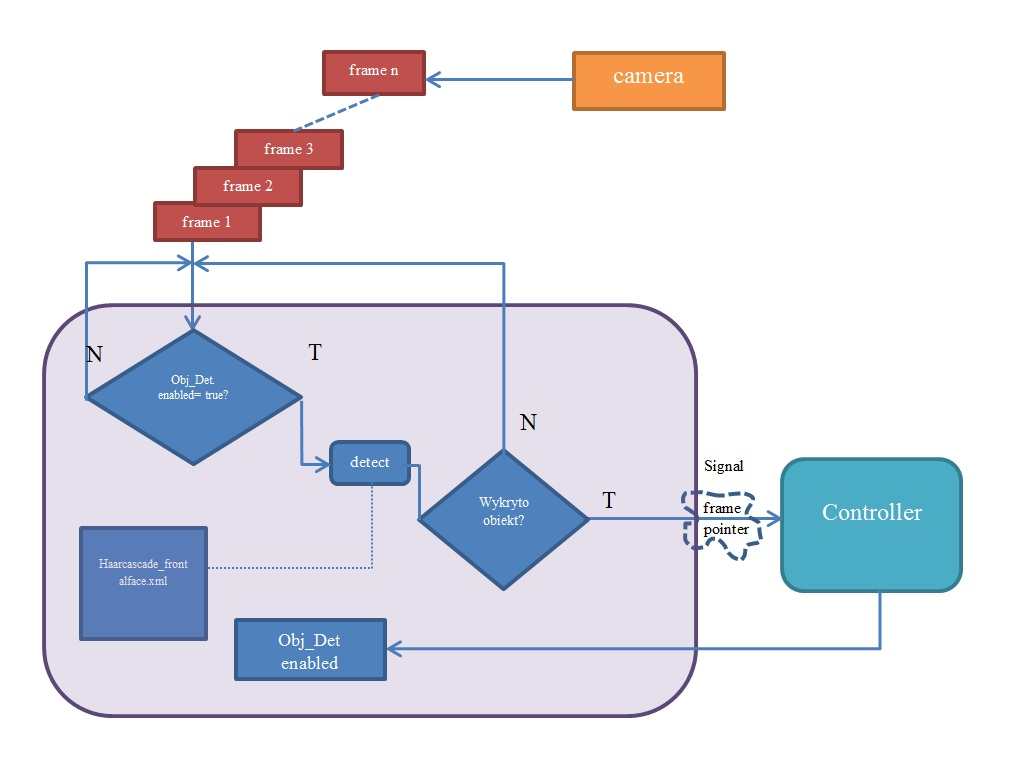
\includegraphics[width=1\linewidth]{sch/detekcja_obj}}
\caption[Schemat działania modułu detekcji obiektów.]{Schemat działania modułu detekcji obiektów .}
\label{fig:detObj}
\end{figure}

\paragraph{Worker} – zadaniem tego modułu jest wykonanie właściwej akcji zadanej przez kamerę. 
W projekcie jest to wystawienie stanu logicznego wysokiego na porcie GPIO, który może przykładowo sterować układem z przekaźnikiem, lub innym układem.
Do implementacji użyto biblioteki wiringPi autorstwa Gordona Hendersona. Biblioteka ta dostarcza łatwy w obsłudze interfejs pozwalający sterować portami GPIO, generować przebiegi PWM, odmierzać czas, oraz wiele innych.
Istotnym zagadnieniem jest mapowanie portów\footnote{Opis mapowania portów znajduje się w dodatku} wirtualnych stosowanych w bibliotece na rzeczywiste wyprowadzenia GPIO.

Na poniższym fragmencie kodu wydruk \ref{Worker} zaprezentowano sposób inicjalizacji biblioteki przez wywołanie funkcji wiringPiSetup(),  a następnie zdefiniowanie portów w konstruktorze klasy Worker.
\paragraph{Logger} - moduł ten odpowiada za wygenerowanie pliku, które skrypty PHP i jQuery po stronie serwera następnie przetwarzają i prezentują użytkownikowi końcowy log. Na listingu \ref{Logger} przedstawiona jest implementacja funkcji roboczej \textbf{work()}.
Moduł rusza do pracy w momencie, gdy obiekt zostanie zdetekowany i zweryfikowany poprawnie.\\
Po otrzymaniu sygnału od \textbf{Controllera} wraz ze wskaźnikiem do struktury \textit{frame} z wykrytym(i) obiektami wywoływana jest robocza funkcja \textbf{work() Loggera}.\\
Kolejnym krokiem jest wyodrębnienie z danej klatki wszystkich twarzy znajdujących się na niej. Do tego wykorzystywany jest wektor \textbf{faces}, w którym to znajdują się współrzędne wszystkich zdetekowanych przez \textbf{Object\_detection} w danej klatce twarzy. W każdej iteracji pętli for tworzona jest oddzielna struktura \textbf{face} typu \textit{Mat} dla każdej twarzy(do tego wykorzystywany jest konstruktor \textit{Mat}, który inicjowany jest klatka \textbf{frame} oraz obszarem zdefiniowanym w wektorze \textbf{faces}, który ma być wyexportowana z \textbf{frame'a}), a następnie generowana jest przez funkcję \textbf{getcurdate()} aktualna data w formacie: [NR\_TWARZY]X[ROK]-[MIESIĄC]-[DZIEŃ]-[GODZINA]:[MINUTA]:[SEKUNDA] , która jest wykorzystana jako nazwa pod, którą zapisywany jest obraz z wyodrębnioną twarzą i rozszerzeniem .jpg. Obrazy zapisywane są w katalogu /var/www/html/faces/. Z tego katalogu skrypt PHP będzie pobierał zdjęcia i przekazywał do skryptu jQuery, aby go następnie przetworzyć i wyświetlić na stronie WWW.
\begin{lstlisting}[caption = {Funkcja robocza klasy Logger.}, label=Logger, language=C++]
extern std::vector<cv::Rect> faces;
bool Logger::work(void* wsk){
	std::cout<<name<<" RUNNING"<<std::endl;
	std::ofstream log;
	frame = (cv::Mat*)(wsk);
#ifdef TIME_TEST
frame = &test_frame;
#endif
	log.open("/var/www/html/log.txt",std::ios::out | std::ios::app);
	if(!log.is_open())
	  std::cout<<"ERROR READING LOG FILE"<<std::endl;

	for(int i=0; i<faces.size();i++){

		//string index = to_string(i);
	    std::string name = getcurdate()+".jpg";
	    cv::Mat face(*frame,faces[i]);
	    std::string str(name);
	    size_t found= str.find_first_of(":");

	    while (found!=std::string::npos)
	     {
	       str[found]='_';
	       found=str.find_first_of(":",found+1);
	     }

	    log<<name<<std::endl;
	    std::string path;
	    path= "/var/www/html/faces/" + str;
	    printf("%s \n",path.c_str());

	    if( !imwrite(path,face))
	    	std::cout<<"ERROR WRITING IMAGE TO FILE"<<std::endl;
	}

return 0;
}
\end{lstlisting}

\begin{lstlisting}[caption = {Konstruktor klasy Worker.}, label=Worker, language=C++]
Worker::Worker(){

	name="WORKER";
#ifdef BRD_BUILD
	wiringPiSetup();
	pinMode (0,OUTPUT);//GPIO_0 (BCM_GPIO 17) (PHYS. HEADER -> 11)
	pinMode (1,INPUT);	//GPIO_1 (BCM_GPIO 18) (PHYS. HEADER -> 12)
#endif
}
     
\end{lstlisting}

Funkcją odpowiedzialną za akcje wykonywane przez moduł Worker jest work(void * wsk) wyrduk \ref{WorkFun}. Jako argument przyjmuje wskaźnik typu void*, który następnie jest konwertowany do zmiennej int state i dekodowany jest rozkaz od Controllera.

\begin{lstlisting}[caption = {Funkcja work klasy Worker}, label=WorkFun, language=C++]
bool Worker::work(void* wsk){

std::cout<<name<<" RUNNING"<<std::endl;
#ifndef TIME_TEST
int state= *(static_cast<int*>(wsk));
#else
int state = 0;
#endif
	if(state == 0){
#ifdef BRD_BUILD
digitalWrite(0,HIGH);
#endif
std::cout<<"WORKER sets HIGH state"<<std::endl; //open door
#ifndef TIME_TEST
SigW(2,wsk);
#endif
}
else if (state == 2){
#ifdef BRD_BUILD
	digitalWrite(0,LOW);
#endif
	std::cout<<"WORKER sets LOW state"<<std::endl; //close door
#ifndef TIME_TEST
	SigW(2,wsk);
#endif
}
else
{}

	return false;
}

\end{lstlisting}

Po wystawieniu stanu moduł przekazuje sterowanie Controllerowi wysyłając sygnał zwrotny SigW wraz z argumentem w postaci otrzymanego na początku wskaźnika wsk.

\section{ Realizacja sprzętowa }
\subsection{Raspberry Pi 2 rev.B}
\subsection{Układ SoC BCM 2836}
\subsection{Moduł kamery}
W podrozdziale omówione zostaną dostępne na rynku rozwiązania, które można wykorzystać w projekcie.  Do kryteriów kluczowych w projekcie należy zaliczyć : szybkość kamery, interfejs komunikacji oraz cenę. 

\paragraph{Kamera  z interfejsem USB}

USB (ang. Universal Serial Bus) – uniwersalny sprzętowy interfejs komunikacyjny opracowany przez firmy Microsoft, Intel, Compaq, IBM i DEC. Wykorzystujący magistralę szeregową o prędkościach transmisji danych odpowiednio w standardach :

\begin{itemize}[noitemsep]
\item USB 1.1 do 12Mbit/s (1,5 MB/s)
\item USB 2.0 do 480 Mbit/s (60MB/s)
\item USB 3.0 do 5 Gbit/s 
\end{itemize}

Moduły z interfejsem USB są dosyć popularne zwłaszcza w rozwiązaniach desktopowych, gdzie szybkość przesyłu danych nie jest kluczowa. Świetnie sprawdzają się jako urządzenia dostarczające strumienia wideo dla aplikacji VoIP (ang. Voice over IP). Jako dodatkowy atut można wyróżnić często stosowane wbudowane mikrofony.
Do zestawienia wybrano popularną kamerę  HD Webcam C310 firmy Logitech. Kamera należy do średniej półki cenowej, jej wybrane parametry przedstawiono poniżej.


\begin{table}[hbt!]
%\myfloatalign
\caption[Podstawowe parametry kamery HD Webcam C310]{Podstawowe parametry kamery HD Webcam C310}
\begin{tabularx}{\textwidth}{|l|X|} 
 \hline
Standard transmisji danych &	Full Speed USB 2.0 \\
Rozdzielczość Video &	320x240(QVGA), 640x480(VGA) \\
Maksymalna ilość klatek/s &	30fps@ 352x288(CIF) 15fps@640x480(VGA) \\
Pole widzenia FOV (ang. Field of View) &	50st. \\
Wbudowany mikrofon &	Tak\\
Cena &	ok. 120zł\\
\hline
\end{tabularx}  
\label{tab:compareAnalysers}
\end{table}


\paragraph{ Dedykowany moduł RaspiCam z interfejsem MIPI CSI-2. } MIPI CSI-2 (Mobile Industry Processor Interface Camera Serial Interface) definiuje jednokierunkowy interfejs między modułem kamery, a procesorem. Pozwala na uzyskanie transmisji danych do 4Gbps ( po 1Gbps na linię danych). Moduł wykorzystywany w projekcie posiada 2 linie, co daje łączną przepustowość na poziomie 2Gbps.
Innym rozwiązaniem jest dedykowany dla platformy Raspberry moduł RaspiCam z  sensorem  OV5647 firmy OmniVision. 

Moduł ten wysyła dane za pomocą szyny Camera Serial Interface (CSI-2) do procesora BCM2835. Wykorzystywana jest do tego złącze taśmowe 15-pinowe podłączane do gniazda CSI Camera płyty Raspberry Pi 2. Według danych producenta kamera jest w stanie dostarczyć strumień wideo o rozdzielczości 1920x1080 przy 30 klatkach na sekundę.

\begin{table}[hbt!]
%\myfloatalign
\caption[Podstawowe parametry kamery RaspiCam]{Podstawowe parametry kamery RaspiCam}
\begin{tabularx}{\textwidth}{|l|X|} 
 \hline
Standard transmisji danych &	MIPI CSI-2 \\
Rozdzielczość Video &	1080p,720p,640x480(VGA) \\
Maksymalna ilość klatek/s &	30fps@ 1080p, 60fps@720p, 90fps@640x480 \\
Pole widzenia FOV (ang. Field of View) & 53.5st. (horizontal) 41.41st (vertical) \\
Wbudowany mikrofon &	Nie \\
Cena: &	85zł \\
\hline
\end{tabularx}  
\label{tab:compareAnalysers}
\end{table}


Tabela 4.2 Podstawowe parametry kamery RaspiCam

Jak widać na korzyść modułu dedykowanego działa nie tylko cena, ale także dużo większa wydajność, wsparcie sprzętowe platformy Raspberry, a przede wszystkim transmisja danych dużo lepsza niż w przypadku kamer z interfejsem USB, co ma wpływ na założoną szybkość kamery. Poniżej znajduje się dokładny opis wybranego modułu RaspiCam.
\begin{description}
\item Sercem modułu jest sensor OV5647 w skład którego wchodzą takie bloki jak :
\begin{itemize}
\item rdzeń sensora optycznego z układami odpowiedzialnymi za przechwycenie obrazu i wstępne przetworzenie go
\item procesor obrazu DPC dokonujący dalszej obróbki
\item interfejs wyjściowy przekształcający dane do odpowiedniego formatu
\end{itemize}
\end{description}
Istotną rolę pełnią bloki generujące sygnały synchronizujące obrazu niezbędne układowi odbierającemu do poprawnego odtworzenia obrazu z danych dostarczonych przez sensor.
Urządzenie komunikuje się z procesorem za pomocą interfejsu SCCB ( ang. Serial Camera Control Bus ). Interfejs ten opiera się na protokole komunikacyjnym I2C (znanym też jako Two Wire Interface) wykorzystującym dwie linie : danych - SDA i zegara – SCL. Urządzenie Master – w tym przypadku procesor BCM2836 wysyła do urządzenia Slave - sensora odpowiednie komunikaty, za pomocą których możliwa jest zmiana jego parametrów.
 

\begin{figure}[bth]
\centering
{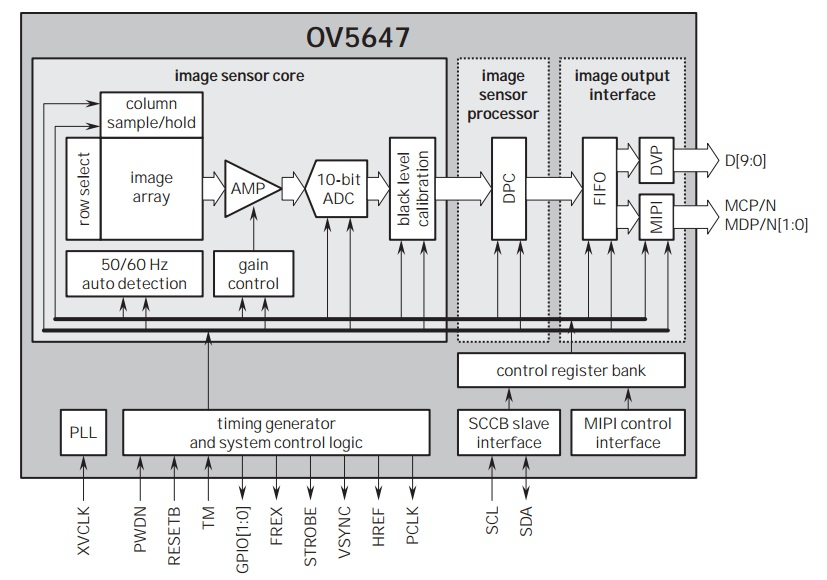
\includegraphics[width=1\linewidth]{sch/OV5647}}
\caption[Schemat funkcjonalny modułu RaspiCam.]{Schemat funkcjonalny modułu RaspiCam.}
\label{fig:detObj}
\end{figure} 

\subsection{Obudowa urządzenia}


	%\include{Chapters/Ch_symulacje}
	% Chapter Ocena działania i skuteczności urządzenia
\chapter{Testowanie} % Chapter title

Jednym z kluczowych zagadnień każdego projektu jest weryfikacja poprawności działania urządzenia. Oprócz weryfikacji funkcjonalnej w pracy tej istotne są pomiary czasów odpowiedzi poszczególnych modułów, a przede wszystkim modułu Object\_Detection odpowiedzialnego za obsługę kamery i przetwarzanie obrazu. Pomiary te pozwolą oszacować całkowity czas odpowiedzi urządzenia, a także dzięki nim będzie można porównać działanie układu opartego na platformie Raspberry i kamerze dedykowanej oraz komputerze klasy PC z kamerą USB.
Na potrzeby procesu testowania zaimplementowane zostały odpowiednie moduły testujące, umożliwiające dzięki zastosowanej przy projektowaniu aplikacji technice OO(orientowanej-obiektowo) w wygodny sposób przeprowadzić scenariusz testowy zaprezentowany na rys.<rysunek>.
\section{Implementacja modułu testowego}
Do przetestowania działania funkcji oraz pomiaru czasu  stworzony został oddzielny moduł Time\_Test. Moduł ten wykorzystuje implementację obiektowo-orientowaną aplikacji głównej, co pozwala w łatwy i przejrzysty sposób dokonać testu i pomiaru czasu działania każdego modułu roboczego.

\begin{lstlisting}[caption = {Klasa testująca}, label=TestClass, language=C++]
class Time_Test{
private:
	int module_nr;
	std::vector <Module*> wektor;

public:
	void add(Module **);
	void measure_time();
	void display_results();
	}; 
\end{lstlisting}

\begin{description}
\item Praca modułu opiera się na trzech funkcjach:
\begin{itemize}[noitemsep]
\item void add(Module**) – metoda ta przyjmuje jako argument tablicę wskaźników na obiekty typu Module i umieszcza je w składowej wektor.
\item bool measure\_time() – metoda odpowiedzialna za pomiar czasów poszczególnych modułów oraz całkowitego. 
\end{itemize}
\item Metoda ta wykorzystuje dostarczone wraz z biblioteką standardową języka C++ bibliotekę chrono, która opiera się na 3 głównych obiektach, jak : 
\begin{itemize}[noitemsep]
\item duration – mierzące okres czasu – w projekcie są to globalne zmienne : time\_span (czas działania modułu), total\_time (czas całkowity) oraz wektor czasów times przechowujący poszczególne czasy działania modułów.
\item time\_point – odniesienie do punktu w czasie – w projekcie są to zmienne t1 oraz t2
\item clock – framework, odpowiadający za odniesienie czasu określonego przez obiekty typu time\_point względem czasu rzeczywistego. – w projekcie są to obiekty typu  time\_point oraz metoda now() zwracająca aktualny czas frameworku high\_resolution\_clock, korzystającego z zegara wysokiej precyzji.

\end{itemize}
\end{description}


\begin{lstlisting}[caption = {Listing Implementacja funkcji testującej}, label=TestFun, language=C++]
void Time_Test::measure_time(int n){

	printf("Start of time tests \n");

	high_resolution_clock::time_point t1;
	high_resolution_clock::time_point t2 ;

	duration<double>  time_span,total_time;
	std::vector <std::chrono::duration<double>> times;
           n=N;
	printf("\nNumber of iterations : %d",n);

		for (int i=0; i<module_nr; ++i){
			 t1 = high_resolution_clock::now();
c=0;
while(c<N){
		 assert(! wektor[i]->work());
c++;
}	
		 	t2 = high_resolution_clock::now();

			 time_span  = duration_cast<nanoseconds>(t2 - t1);
			 times.push_back(time_span);
			 total_time += time_span;
		  } 

\end{lstlisting}

Funkcja przedstawiona na listingu 5.2 posiada pętlę główną for – w ramach której następuje iteracja po kolejnych modułach i wywołanie polimorficzne funkcji work() dla każdego z nich. Wywołanie to jest objęte dodatkową pętlą while, która jest odpowiedzialna za uśrednienie wyników pomiaru czasu. W każdej iteracji pętli for funkcja ta zapisuje w zmiennych t1 i t2 punkty czasowe odpowiednio przed i po wywołaniu N-razy (n jest argumentem wejściowym wywołania programu głównego) funkcji składowej work() badanego modułu, a następnie zapisuje wartość ich różnicy do zmiennej time\_span. Czas zmierzony dla każdego modułu jest umieszczony w wektorze times. Jednocześnie w zmiennej total\_time przechowywany jest czas całkowity wykonania sekwencji modułów.

Metoda ta dokonuje także testu poprawności działania funkcji. Polega to na wywołaniu każdej funkcji roboczej work() modułów wewnątrz funkcji assert().
Jeśli funkcja work zwróci wartość różną od 0 to funkcja assert poda komunikat wraz z nazwą pliku źródłowego i numeru linii w której to się stało.

Za pomocą metody display\_results() wyniki  przechowywane w wektorze times i zmiennej total\_time są uśrednione i prezentowane użytkownikowi dla każdego modułu.

\section{ Wyniki pomiarów}
W tabeli 5.1 znajduje się zestawienie pomiarów czasów wykonanych na platformie Raspberry Pi 2 z modułem RaspiCam oraz na komputerze klasy notebook: ASUS  X53S z modułem kamery USB.
Specyfikacja platformy ASUS:
\begin{itemize}[noitemsep]
\item Procesor Inter Core i5 2410M
\item Pamięć 8GB 1333MHz DDR3
\item GPU: Nvidia GeForce GT 540M 1GB DDR3
\item Dysk twardy 750GB SATA 7200 obr./min.
\end{itemize}
Systemem wykorzystanym na platformie ASUS jest Linux Ubuntu 14.04 uruchamianym w maszynie wirtualnej programu VirtualBox (wersja 4.3.30). 
Zasoby przydzielone maszynie wirtualnej :
\begin{itemize}[noitemsep]
\item 4GB pamięci RAM
\item 2 wirtualne rdzenie CPU
\item 128 MB Video Memory
\end{itemize}
Specyfikacja platformy Raspberry :
\begin{itemize}[noitemsep]
\item Procesor BCM 2836  quad core
\item 1GB pamięci RAM DDR2
\item GPU: VideoCore IV (przydzielone 128 MB pamięci RAM z zasobów wspólnych)
\end{itemize}
Poniżej znajdują się wyniki dla N = 10, 100 i 500 powtórzeń wywołania funkcji roboczych poszczególnych modułów dla rozdzielczości strumienia : 320x240.

\begin{table}[hbt!]
%\myfloatalign
\caption[Ilość iteracji N = 10]{Zestawienie wyników pomiarów czasu dla różnych wartości N. Ilość iteracji N = 10}
\begin{tabularx}{\textwidth}{|l|X|X|} 
 \hline
Moduł&	ASUS x53S&	Raspberry Pi 2\\ \hline
Object\_Detection [ms]	&254,762741&	549,6572\\
Worker [us]	&832,679&	98,599\\
Logger [ms]	&0,712403&	6,425799\\
Całkowity średni czas [ms]&	256&	556 \\
\hline
\end{tabularx}  
\label{tab:compareAnalysers}
\end{table}


\begin{table}[hbt!]
%\myfloatalign
\caption[Ilość iteracji N = 100]{Zestawienie wyników pomiarów czasu dla różnych wartości N. Ilość iteracji N = 100}
\begin{tabularx}{\textwidth}{|l|X|X|} 
 \hline
Moduł&	ASUS x53S	&Raspberry Pi 2 \\ \hline
Object\_Detection [ms]&	137,7835103	&523,30284 \\
Worker [us]	&387,455	&80,37 \\
Logger [ms]&	1,907358&	6,440570 \\
Całkowity średni czas [ms]	&140&	529 \\
\hline
\end{tabularx}  
\label{tab:compareAnalysers}
\end{table}


\begin{table}[hbt!]
%\myfloatalign
\caption[Ilość iteracji N = 500]{Zestawienie wyników pomiarów czasu dla różnych wartości N. Ilość iteracji N = 500}
\begin{tabularx}{\textwidth}{|l|X|X|} 
 \hline
Moduł&	ASUS x53S	&Raspberry Pi 2\\ \hline
Object\_Detection [ms]&	118,555288	&525,432592\\
Worker [us]&	95,112&	77,03\\
Logger [ms]&	1,339017&	6,264304\\
Całkowity średni czas [ms]&	119&	531\\
\hline
\end{tabularx}  
\label{tab:compareAnalysers}
\end{table}

\section{Uruchomienie testów}
\begin{description}
\item Na proces testowania składa się:
\begin{itemize}[noitemsep]
\item Zbudowanie projektu 
\item Załadowanie modułu sterownika V4L2
\item Uruchomienie aplikacji testowej z odpowiednimi argumentami
\end{itemize}
\end{description}
Na zbudowanie projektu składają się min. Kompilacja warunkowa ( zbędne do testowania bloki aplikacji głównej są pomijane), oraz wywołanie skryptu budującego makefile.
Załadowanie sterownika możliwe jest z poziomu linii komend i musi być koniecznie wykonane przed uruchomieniem aplikacji. Minimalna wersja komendy ta jest następująca:\\
uv4l $--$driver raspicam $--$video\_nr nr\\
Gdzie nr to index pod jakim zostanie zarejestrowane urządzenie RaspiCam przez sterownik V4L2 w systemie (np. dla nr = 0 będzie to : /dev/video0).\\
Dodatkowe argumenty pozwalające konfigurować sensor z poziomu sterownika to :\\
$--$encoding yuv420\\
$--$width 320\\
$--$height 240\\
Atrybut $--$encoding pozwala wymusić format kodowania obrazu, w tym przypadku zastosowany jest format YUV420. Kolejne dwa argumenty są odpowiedzialne za szerokość i wysokość obrazu strumienia(w projekcie można je pominąć z  uwagi na to, że z poziomu aplikacji także są konfigurowalne, co jest opisane niżej oraz w rozdziale 4.).\\  
Uruchomienie wymaga podania ścieżki pliku binarnego cam wraz z argumentami oddzielonymi spacjami:\\
./cam width height N\\
width – szerokość klatki strumienia video\\
height – wysokość klatki strumienia video\\
N – ilość iteracji ( opisane w paragrafie 5.2)\\
Przykładowe wywołanie : ./cam 320 240 100\\
Uruchomi w rezultacie aplikację testową z parametrami strumienia : rozdzielczość 320x240 oraz wykona uśrednione na 100 iteracjach testy.

\section{Wnioski}
Na podstawie pomiarów stwierdzić można, że kamera zrealizowana na platformie Raspberry ustępuje urządzeniu o dużo większej mocy obliczeniowej jakim jest laptop ASUS x53S.
Jak widać przy większej ilości iteracji średnie czasy są znacznie mniejsze. W przypadku platformy ASUS wyraźnie widać względny spadek czasów. Najprawdopodobniej wynika to z optymalizacji sprzętowej procesora i jednostki GPU przy wielokrotnym odnoszeniu się do tego samego fragmentu pamięci.
W obu przypadkach na całkowity czas odpowiedzi kamery ma wpływ głównie działanie modułu Object\_Detection. Nie jest to zaskakujący rezultat, gdyż moduł ten wykonuje dwa ważne zadania tj. pośredniczy w przechwyceniu strumienia video oraz dokonuje przetworzenia każdej przez algorytm wykorzystujący kaskady Haar’a. Zdecydowana przewaga platformy ASUS wynika z dużo większej wydajności jednostki GPU i CPU względem platformy Raspberry. Dla pomiaru czasu działania modułu Logger’a kluczowym aspektem jest nośnik na jakim dokonywany jest zapis zdjęcia wykrytego obiektu. 
Raspberry Pi 2 wykorzystuje kartę Micro SD class 10, co wg specyfikacji powinno gwarantować minimalny transfer na poziomie 10MB/s. W przypadku ASUS’a jest to dużo szybszy dysk twardy wykorzystujący magistralę SATA, zapewniającą wg specyfikacji transfer na poziomie ok. 179MB/s. Stąd też widoczna jest róznica w czasach.
Jako, że laptop ASUS nie posiada portów GPIO, test modułu Worker w zasadzie pokazuje tylko czas wywołania funkcji roboczej.\\
Podsumowując – platforma Raspberry pod względem wydajności ustępuje rozwiązaniom desktopowym, jednak różnica nie jest ogromna. Czas reakcji na poziomie 0,5s z powodzeniem pozwala na wykorzystanie urządzenia w wielu dziedzinach.
\begin{description}
\item Ponadto uwzględniając atuty takie jak:
\begin{itemize}
 \item niewielkie gabaryty
 \item niskie zużycie energii
 \item możliwość sterowania urządzeniami zewnętrznymi 
 \item mobilność - łatwość montażu w warunkach trudno dostępnych
 \item niską cenę
 \item możliwość własnej implementacji sprzętowej (przygotowanie dedykowanego urządzenia na podstawie płyty bazowej)
  
 Raspberry Pi 2 zdecydowanie wygrywa z platformą ASUS.
\end{itemize}
\end{description}

%Podsumowanie ma być jako nowy rozdział (chapter!)
\chapter{Podsumowanie} 

Realizacja pracy zakończyła się sukcesem. Kamera spełnia wszystkie założenia i jest zgodna z obraną koncepcją. Potwierdzeniem tego są wykonane testy, które zweryfikowały projekt jako poprawnie działający, a do tego pokazały realne możliwości sprzętowo-programowe urządzenia.\\
Niniejsza praca jest doskonałą bazą wyjściową do dalszego rozwoju. Dzięki zaimplementowanej elastycznej strukturze aplikacji możliwe jest rozszerzenie funkcjonalności o komunikację z innymi urządzeniami i stworzenie sieci kamer współpracujących ze sobą. A także adaptację innych algorytmów na potrzeby np. diagnostyki medycznej, czy zastosowań w robotyce.	

%----------------------------------------------------------------------------------------
%	BIBLIOGRAPHY, CONTENSTS, LISTS
%----------------------------------------------------------------------------------------
	%%%%%%%%%%%%%%%%%%%%%%%%%%%%%%%%%%%%%%%%%%%%%%%%%%%%%%%%%%%%%  
% BIBLIOGRAFIA
%%%%%%%%%%%%%%%%%%%%%%%%%%%%%%%%%%%%%%%%%%%%%%%%%%%%%%%%%%%%%%
\begin{thebibliography}{99}
\bibitem{PodstawySystemów} Abraham Silberschatz, Peter B.Galvin, Greg Gagne {\it Podstawy systemów operacyjnych }\\ Wydawnictwo Naukowo-Techniczne, 2005 \\
\bibitem{LinuxWsystemachEmbedded} Marcin Bis {\it Linux w systemach embedded }\\ Wydawnictwo BTC, 2011 \\
\bibitem{Symfonia} Jerzy Grębosz {\it Symfonia C++}\\ Wydawnictwo Oficyna Kallimach, 2010 \\
\bibitem{LinuxProgSys} Robert Love {\it Linux programowanie systemowe. Przewodnik po jądrze systemu Linux}\\ Wydawnictwo Helion, 2013 \\

\bibitem{Boost} Boost Library Project, Boost Library, dokumentacja techniczna  \\
		\url{http://boost.org/doc/}\\
\bibitem{UV4L} Luca Risolia, User-space Video for Linux driver  \\
		\url{http://www.linux-projects.org/modules/sections/}, \\
\bibitem{WiringPi}  Gordon Henderson, GPIO Interface library for the Raspberry Pi\\
		\url{http://www.wiringpi.com/} \\
\bibitem{Apache} The Apache Software Foundation, Apache 2 HTTP Server, dokumentacja techniczna.\\
		\url{http://httpd.apache.org/docs/} \\
\bibitem{Raspberry}Raspberry Pi Foundation, Raspberry Pi dokumentacja  \\
		\url{http://raspberrypi.org/} \\ 
%		\url{http://moto.wp.pl/kat,106078,title,General-Motors-400-000-aut-wezwanych-do-naprawy,wid,16719519,wiadomosc.html?ticaid=113c5c#stgOpinie} General Motors 400 000 aut wezwanych do naprawy. 2014.06.29
\bibitem{haydenjames} Raspberry Pi 2 Overclock.Hayden James 6 Luty 2015 \\
		\url{http://haydenjames.io/raspberry-pi-2-overclock/} \\						
							
\bibitem{Apacheconfig} How to install Apache, MySQL,PHP stack on Ubuntu, \\
	\url{https://www.digitalocean.com/community/tutorials/} \\ 
	
\end{thebibliography}

	
%----------------------------------------------------------------------------------------
%	APENDIX
%----------------------------------------------------------------------------------------
	\appendix
	% Chapterd Dodatek A
\chapter{Mapowanie portów procesora BCM2836} % Chapter title

\label{ch:BCM2836} % For referencing the chapter elsewhere, use \autoref{ch:name} 

Mapowanie portów procesora BCM2836 
Wyprowadzenia portów GPIO na płycie są identyczne w przypadku płyt Raspberry Pi, Raspberry Pi rev. B i Raspberry Pi 2 rev. B – jest to 40 złączy typu goldpin. Jednak wraz ze zmianą jednostek SoC w poszczególnych wersjach płyt zmianie uległy też rozkład i funkcje odpowiednich pinów.
Biblioteka wiringPi dostarcza wygodny interfejs obsługi portów GPIO układów z rodziny Raspberry Pi, dzięki któremu programista nie musi sprawdzać tych portów, zapewniając przenośność kodu między różnymi wersjami urządzeń.
 Autor biblioteki proponuje własny schemat numeracji pinów rozpoczynający się od GPIO0 do GPIO7 na głównym złączu P1. Oprócz tego dostępne są też porty specjalnego przeznaczenia jak np. złącza SDA i SCL interfejsu I2C.

\begin{figure}[bth]
\centering
{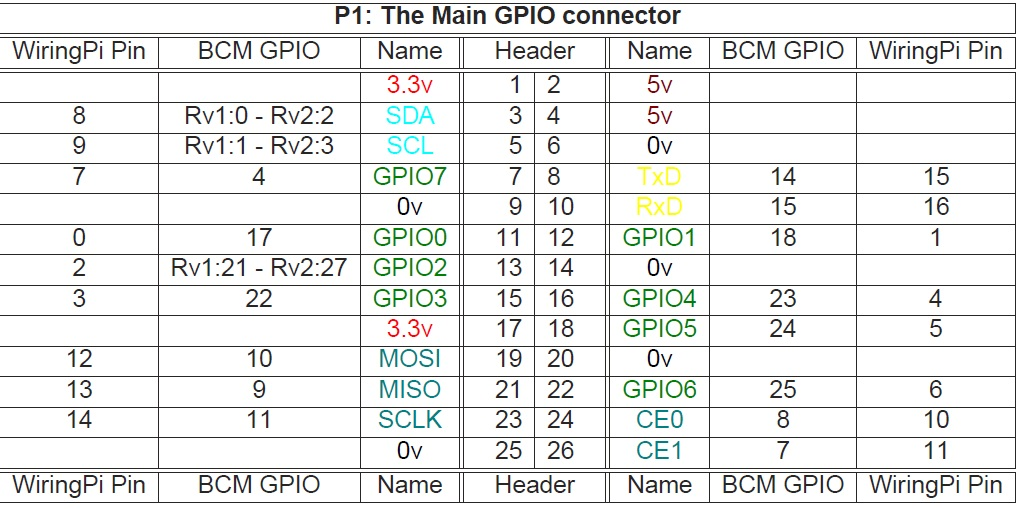
\includegraphics[width=1\linewidth]{sch/pinMap}}
\caption[Mapowanie portów GPIO biblioteki wiringPi.]{Mapowanie portów GPIO biblioteki wiringPi.}
\label{fig:detObj}
\end{figure} 
	%\include{Chapters/Dodatek_B}	%karta SD
	%\include{Chapters/Dodatek_C}
	%\include{Chapters/Dodatek_D}	%SP601
	%\include{Chapters/Dodatek_E}	%SP601
%----------------------------------------------------------------------------------------
%	TikZ diagrams, charts, diagramflow ect..
%----------------------------------------------------------------------------------------
	%
%-------------------------------------------------------------------------------
% Pie chart - color
%-------------------------------------------------------------------------------
\begin{figure}
\centering
\def\angle{0}
\def\radius{3}
\def\cyclelist{{"orange","blue","red","green"}}
\newcount\cyclecount \cyclecount=-1
\newcount\ind \ind=-1
\begin{tikzpicture}[nodes = {font=\sffamily}]
  \foreach \percent/\name in {
      46.6/Chrome,
      24.6/Internet Explorer,
      20.4/Firefox,
      5.1/Safari,
      1.3/Opera,
      2.0/Other
    } {
      \ifx\percent\empty\else               % If \percent is empty, do nothing
        \global\advance\cyclecount by 1     % Advance cyclecount
        \global\advance\ind by 1            % Advance list index
        \ifnum3<\cyclecount                 % If cyclecount is larger than list
          \global\cyclecount=0              %   reset cyclecount and
          \global\ind=0                     %   reset list index
        \fi
        \pgfmathparse{\cyclelist[\the\ind]} % Get color from cycle list
        \edef\color{\pgfmathresult}         %   and store as \color
        % Draw angle and set labels
        \draw[fill={\color!50},draw={\color}] (0,0) -- (\angle:\radius)
          arc (\angle:\angle+\percent*3.6:\radius) -- cycle;
        \node at (\angle+0.5*\percent*3.6:0.7*\radius) {\percent\,\%};
        \node[pin=\angle+0.5*\percent*3.6:\name]
          at (\angle+0.5*\percent*3.6:\radius) {};
        \pgfmathparse{\angle+\percent*3.6}  % Advance angle
        \xdef\angle{\pgfmathresult}         %   and store in \angle
      \fi
    };
\end{tikzpicture}
\caption{Pie chart}
\end{figure}

%-------------------------------------------------------------------------------
% Circular arrows with text
%-------------------------------------------------------------------------------
\begin{figure}
\centering
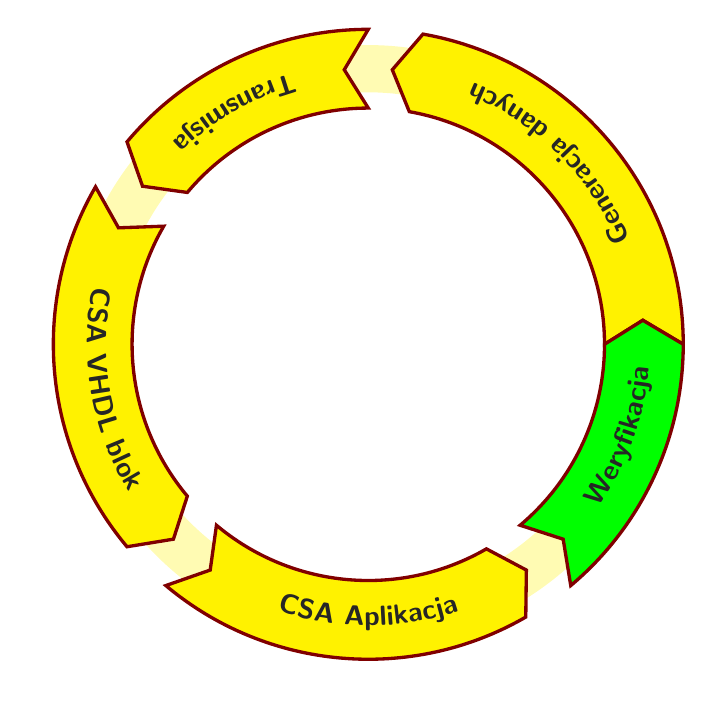
\begin{tikzpicture}
  \fill[even odd rule,yellow!30] circle (3.8) circle (3.2);
%  \foreach \x in {0,60,...,300} {
%    \arcarrow{3}{3.5}{4}{\x+20}{\x+100}{5}{red,
%      draw = red!50!black, very thick}{napisr \x}
%  }
	
	\arcarrow{3}{3.5}{4}{0}{80}{5}{yellow,
      draw = red!50!black, very thick}{Generacja danych}
    \arcarrow{3}{3.5}{4}{90}{140}{5}{yellow,
      draw = red!50!black, very thick}{Transmisja}
    \arcarrow{3}{3.5}{4}{150}{220}{5}{yellow,
      draw = red!50!black, very thick}{CSA VHDL blok}
    \arcarrow{3}{3.5}{4}{230}{300}{5}{yellow,
      draw = red!50!black, very thick}{CSA Aplikacja}
    \arcarrow{3}{3.5}{4}{310}{360}{5}{green,
      draw = red!50!black, very thick}{Weryfikacja}
\end{tikzpicture}
\caption{Circular arrows with text}
\end{figure}
%-------------------------------------------------------------------------------

%-------------------------------------------------------------------------------
% Inertial navigation system
%-------------------------------------------------------------------------------
% We need layers to draw the block diagram
\pgfdeclarelayer{background}
\pgfdeclarelayer{foreground}
\pgfsetlayers{background,main,foreground}

% Define a few styles and constants
\tikzstyle{sensor}=[draw, fill=blue!20, text width=5em, 
    text centered, minimum height=2.5em]
\tikzstyle{ann} = [above, text width=5em]
\tikzstyle{naveqs} = [sensor, text width=6em, fill=red!20, 
    minimum height=12em, rounded corners]
\def\blockdist{2.3}
\def\edgedist{2.5}

\begin{figure}
\centering
\begin{tikzpicture}
    \node (naveq) [naveqs] {Wishbone \\ bus};
    % Note the use of \path instead of \node at ... below. 
    \path (naveq.140)+(-\blockdist,0) node (gyros) [sensor] {Acqusition};
    \path (naveq.-150)+(-\blockdist,0) node (accel) [sensor] {rs232syscon};
    
    % Unfortunately we cant use the convenient \path (fromnode) -- (tonode) 
    % syntax here. This is because TikZ draws the path from the node centers
    % and clip the path at the node boundaries. We want horizontal lines, but
    % the sensor and naveq blocks aren't aligned horizontally. Instead we use
    % the line intersection syntax |- to calculate the correct coordinate
    \path [draw, ->] (gyros) -- node [above] {$\vc{\omega}_{ib}^b$} 
        (naveq.west |- gyros) ;
    % We could simply have written (gyros) .. (naveq.140). However, it's
    % best to avoid hard coding coordinates
    \path [draw, ->] (accel) -- node [above] {$\vc{f}^b$} 
        (naveq.west |- accel);
    \node (IMU) [below of=accel] {IMU};
    \path (naveq.south west)+(-0.6,-0.4) node (INS) {INS};
    \draw [->] (naveq.50) -- node [ann] {Velocity } + (\edgedist,0) 
        node[right] {$\vc{v}^l$};
    \draw [->] (naveq.20) -- node [ann] {Attitude} + (\edgedist,0) 
        node[right] { $\mx{R}_l^b$};
    \draw [->] (naveq.-25) -- node [ann] {Horisontal position} + (\edgedist,0)
        node [right] {$\mx{R}_e^l$};
    \draw [->] (naveq.-50) -- node [ann] {Depth} + (\edgedist,0) 
        node[right] {$z$};
    
    % Now it's time to draw the colored IMU and INS rectangles.
    % To draw them behind the blocks we use pgf layers. This way we  
    % can use the above block coordinates to place the backgrounds   
    \begin{pgfonlayer}{background}
        % Compute a few helper coordinates
        \path (gyros.west |- naveq.north)+(-0.5,0.3) node (a) {};
        \path (INS.south -| naveq.east)+(+0.3,-0.2) node (b) {};
        \path[fill=yellow!20,rounded corners, draw=black!50, dashed]
            (a) rectangle (b);
        \path (gyros.north west)+(-0.2,0.2) node (a) {};
        \path (IMU.south -| gyros.east)+(+0.2,-0.2) node (b) {};
        \path[fill=blue!10,rounded corners, draw=black!50, dashed]
            (a) rectangle (b);
    \end{pgfonlayer}
\end{tikzpicture}
\caption{Circular arrows with text}
\end{figure}

%-------------------------------------------------------------------------------

%-------------------------------------------------------------------------------
% State machine
%-------------------------------------------------------------------------------
\begin{figure}
\centering
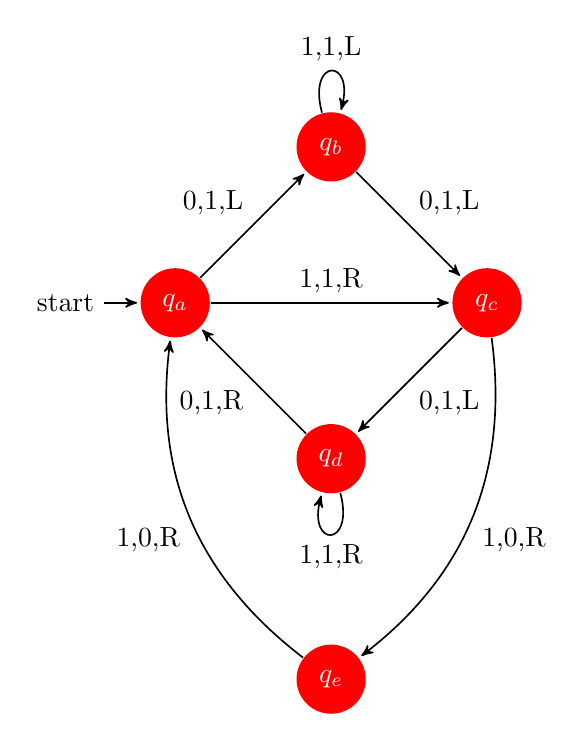
\begin{tikzpicture}[->,>=stealth',shorten >=1pt,auto,node distance=2.8cm,
                    semithick]
  \tikzstyle{every state}=[fill=red,draw=none,text=white]

  \node[initial,state] (A)                    {$q_a$};
  \node[state]         (B) [above right of=A] {$q_b$};
  \node[state]         (D) [below right of=A] {$q_d$};
  \node[state]         (C) [below right of=B] {$q_c$};
  \node[state]         (E) [below of=D]       {$q_e$};

  \path (A) edge              node {0,1,L} (B)
            edge              node {1,1,R} (C)
        (B) edge [loop above] node {1,1,L} (B)
            edge              node {0,1,L} (C)
        (C) edge              node {0,1,L} (D)
            edge [bend left]  node {1,0,R} (E)
        (D) edge [loop below] node {1,1,R} (D)
            edge              node {0,1,R} (A)
        (E) edge [bend left]  node {1,0,R} (A);
\end{tikzpicture}
\caption{State machine}
\end{figure}
%-------------------------------------------------------------------------------

%-------------------------------------------------------------------------------
% Computer science mindmap
%-------------------------------------------------------------------------------

\begin{figure}
\centering
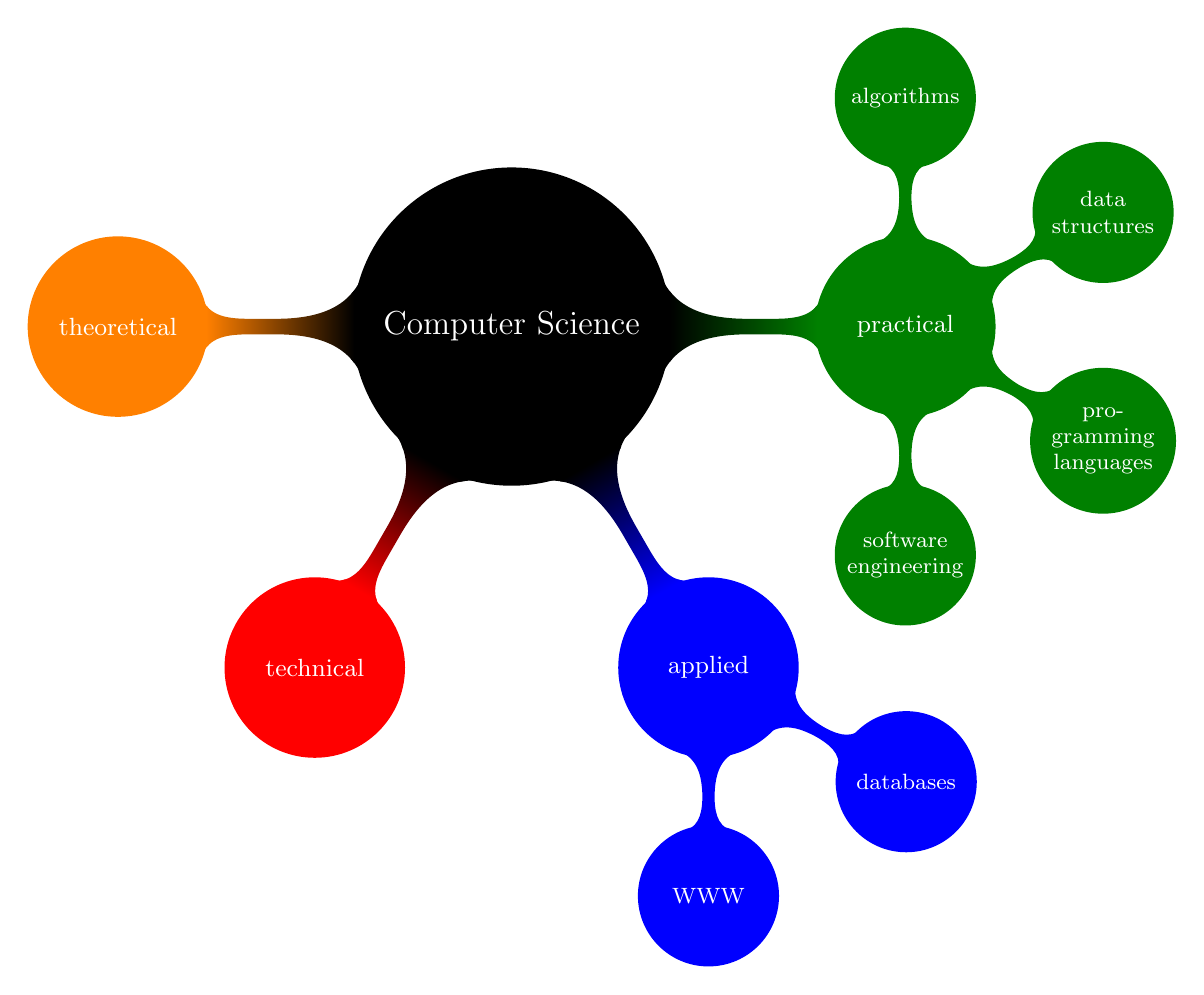
\begin{tikzpicture}
  \path[mindmap,concept color=black,text=white]
    node[concept] {Computer Science}
    [clockwise from=0]
    child[concept color=green!50!black] {
      node[concept] {practical}
      [clockwise from=90]
      child { node[concept] {algorithms} }
      child { node[concept] {data structures} }
      child { node[concept] {pro\-gramming languages} }
      child { node[concept] {software engineer\-ing} }
    }  
    child[concept color=blue] {
      node[concept] {applied}
      [clockwise from=-30]
      child { node[concept] {databases} }
      child { node[concept] {WWW} }
    }
    child[concept color=red] { node[concept] {technical} }
    child[concept color=orange] { node[concept] {theoretical} };
\end{tikzpicture}
\caption{State machine}
\end{figure}
%-------------------------------------------------------------------------------

\begin{figure}[hbt!]
\centering
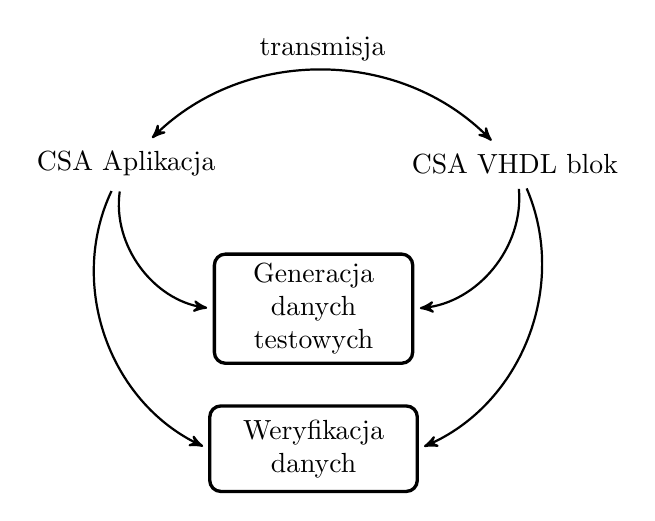
\begin{tikzpicture}[node distance=1cm, auto,]
 %nodes
 \node[punkt] (market) {Generacja danych testowych};
 \node[punkt, inner sep=5pt,below=0.5cm of market]
 (formidler) {Weryfikacja danych};
 % We make a dummy figure to make everything look nice.
 \node[above=of market] (dummy) {};
 \node[right=of dummy] (t) {CSA VHDL blok}
   edge[pil,bend left=45] (market.east) % edges are used to connect two nodes
   edge[pil, bend left=45] (formidler.east); % .east since we want
    ;                                         % consistent style
 \node[left=of dummy] (g) {CSA Aplikacja}
   edge[pil, bend right=45] (market.west)
   edge[pil, bend right=45] (formidler.west)
   edge[pil,<->, bend left=45] node[auto] {transmisja} (t);
\end{tikzpicture}
\caption{Schemat scenariusza testowego.}
\label{fig:circ_arrow}
\end{figure}

%----------------------------------------------------------------------------------------
\end{document}
